\chapter*{Le trek du Salkantay vers le Machu Picchu\markboth{Le trek du Salkantay vers le Machu Picchu}{}}
\section*{2 juin 2015}

Le trek du Salkantay en 6 jours (4 jours de trek, 1 jour pour visiter le Machu Picchu et un jour pour rentrer) : 174 dollars tout inclus avec l'option pour monter en haut de la montagne du Machu Picchu.

\subsection*{Jour 1}
Trajet Cusco-Mollepata en bus puis en camion jusqu'au départ du trek. 

\begin{center} 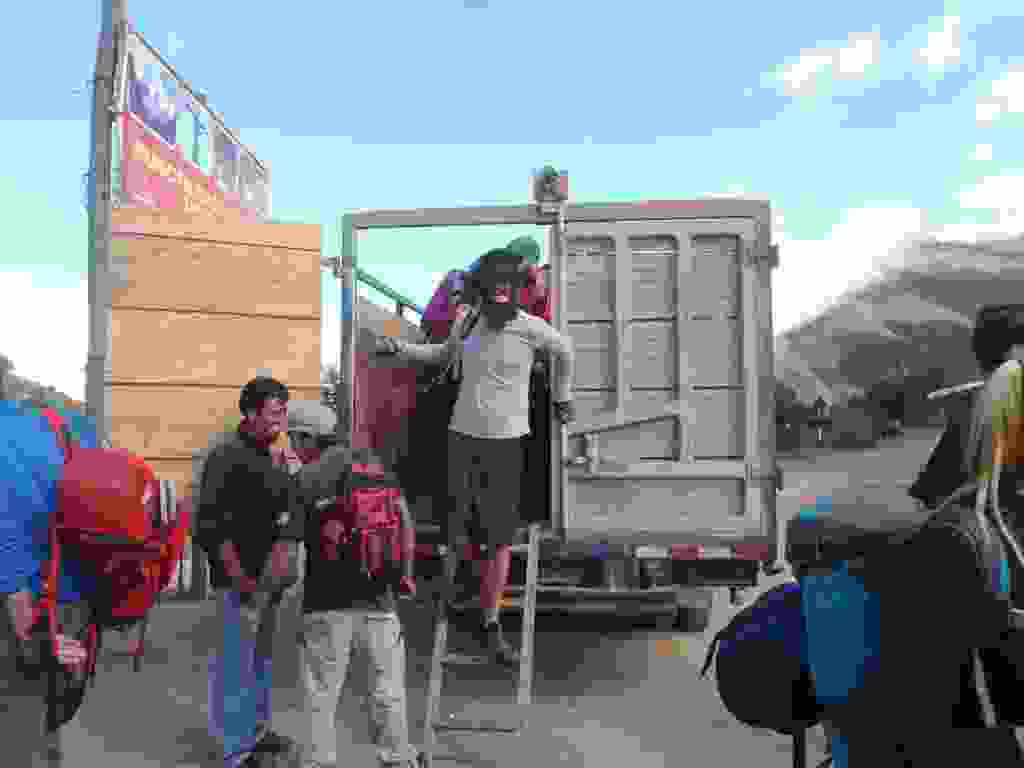
\includegraphics[width=\mywidth]{../wp-content/uploads/2015/05/P5234337-1024x768.jpg} \end{center}
\vspace{-\topsep}
\vspace{-1mm}
\pagebreak

Belle montée pour atteindre le premier campement à 3900m. 
\begin{center} 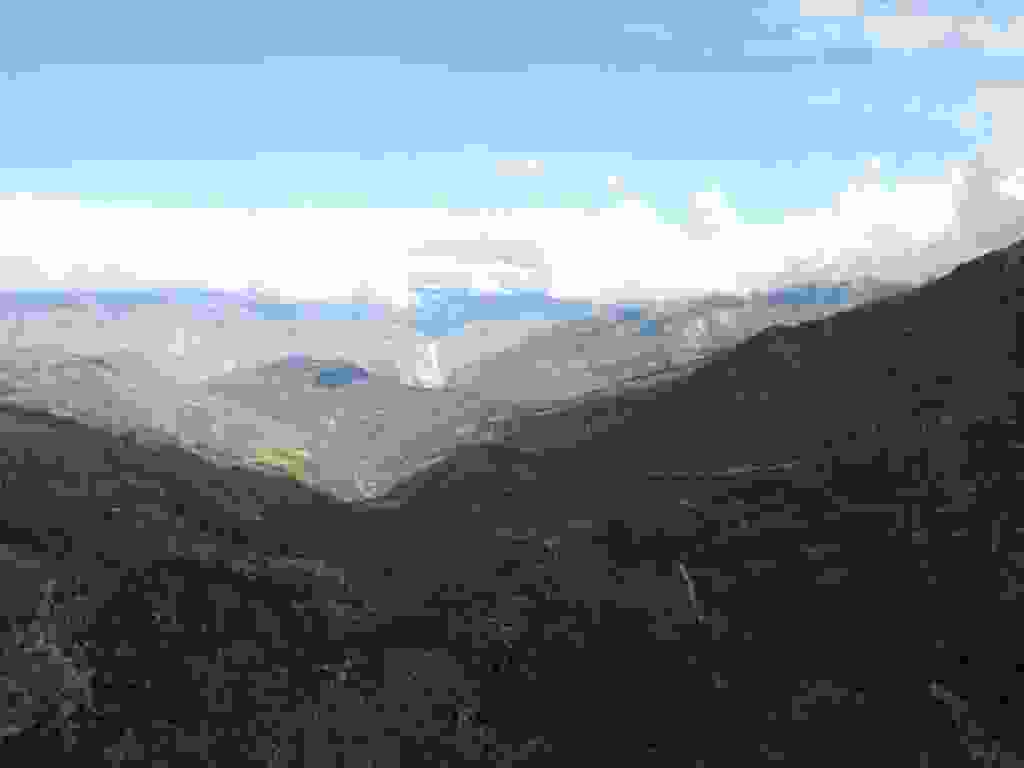
\includegraphics[width=\mywidth]{../wp-content/uploads/2015/05/P5234342-1024x768.jpg} \end{center}
~
\begin{center} 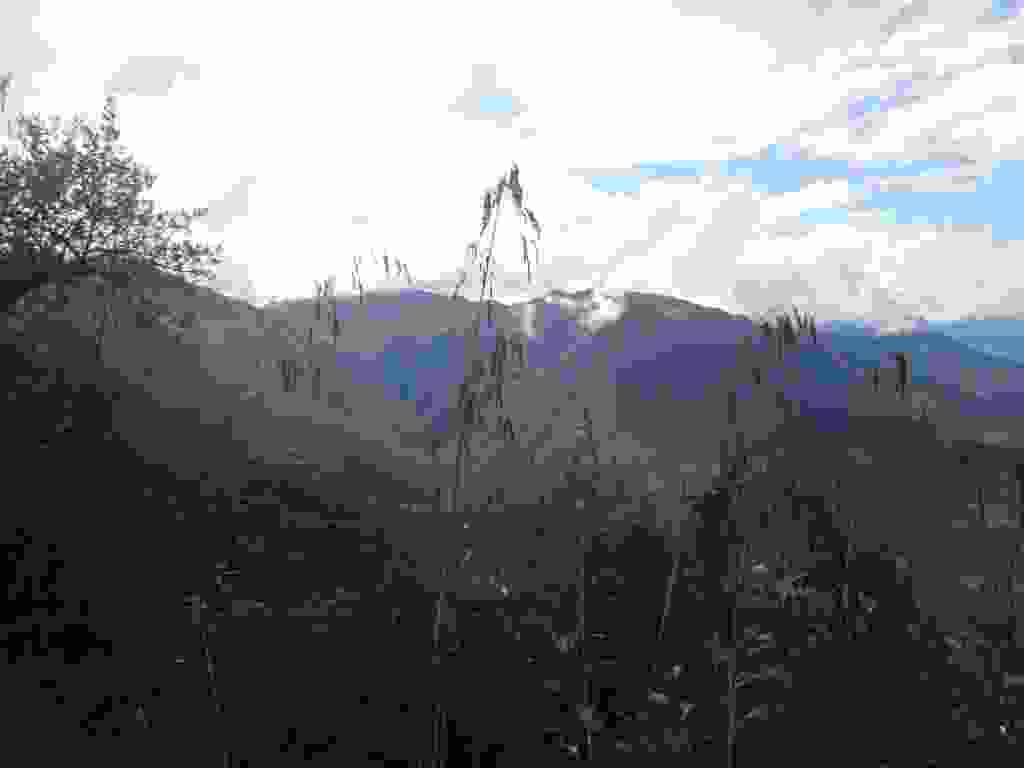
\includegraphics[width=\mywidth]{../wp-content/uploads/2015/05/P5234343-1024x768.jpg} \end{center}
\vspace{-\topsep}
\pagebreak
~
\begin{center} 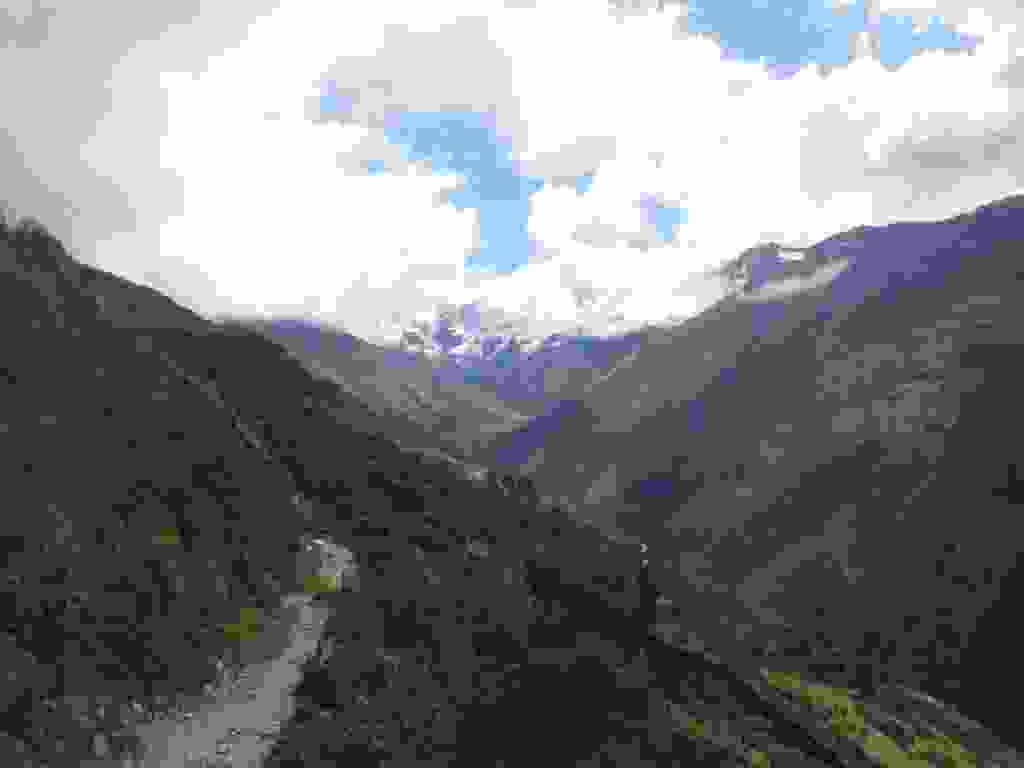
\includegraphics[width=\mywidth]{../wp-content/uploads/2015/05/P5234346-1024x768.jpg} \end{center}

On commence à voir le glacier du Salkantay. 
\begin{center} 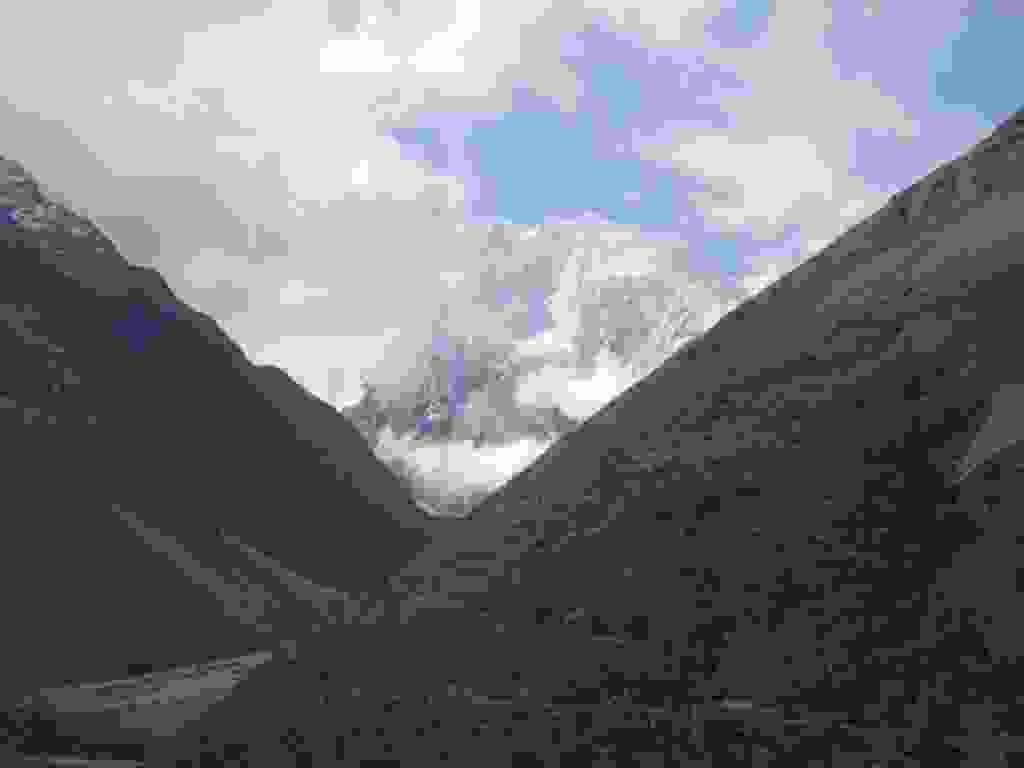
\includegraphics[width=\mywidth]{../wp-content/uploads/2015/05/P5234353-1024x768.jpg} \end{center}
\vspace{-\topsep}
\pagebreak

L'après-midi aller-retour pour voir un lac au pied du glacier Umantay. 
\begin{center} 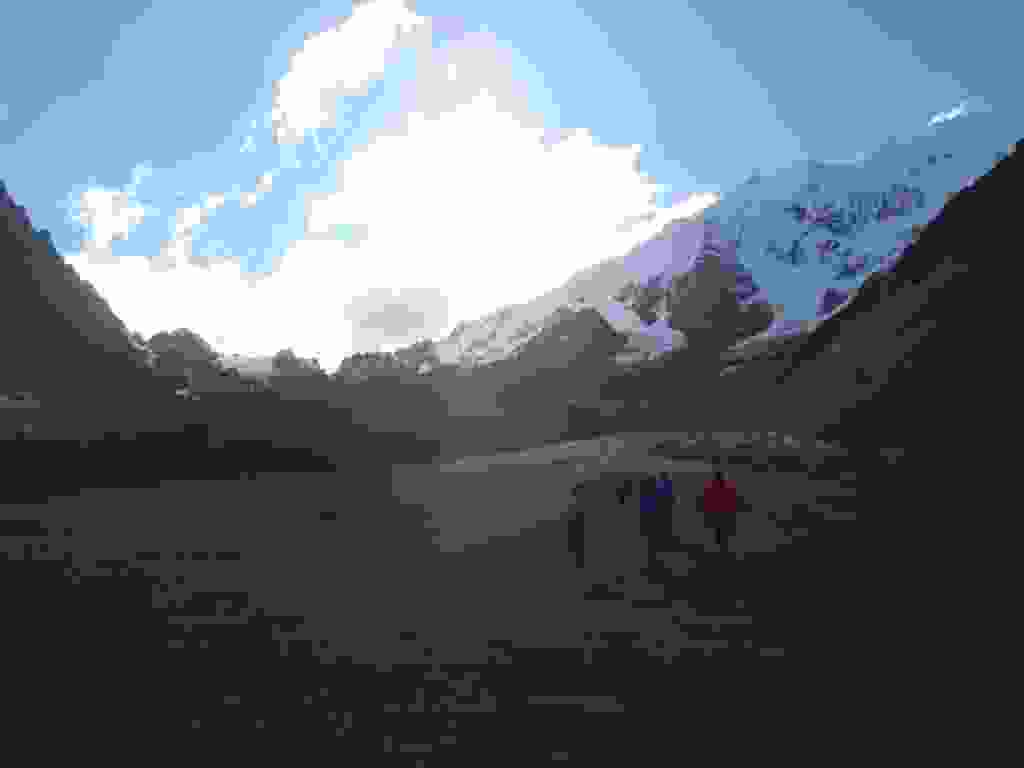
\includegraphics[width=\mywidth]{../wp-content/uploads/2015/05/P5234357-1024x768.jpg} \end{center}
\begin{center} 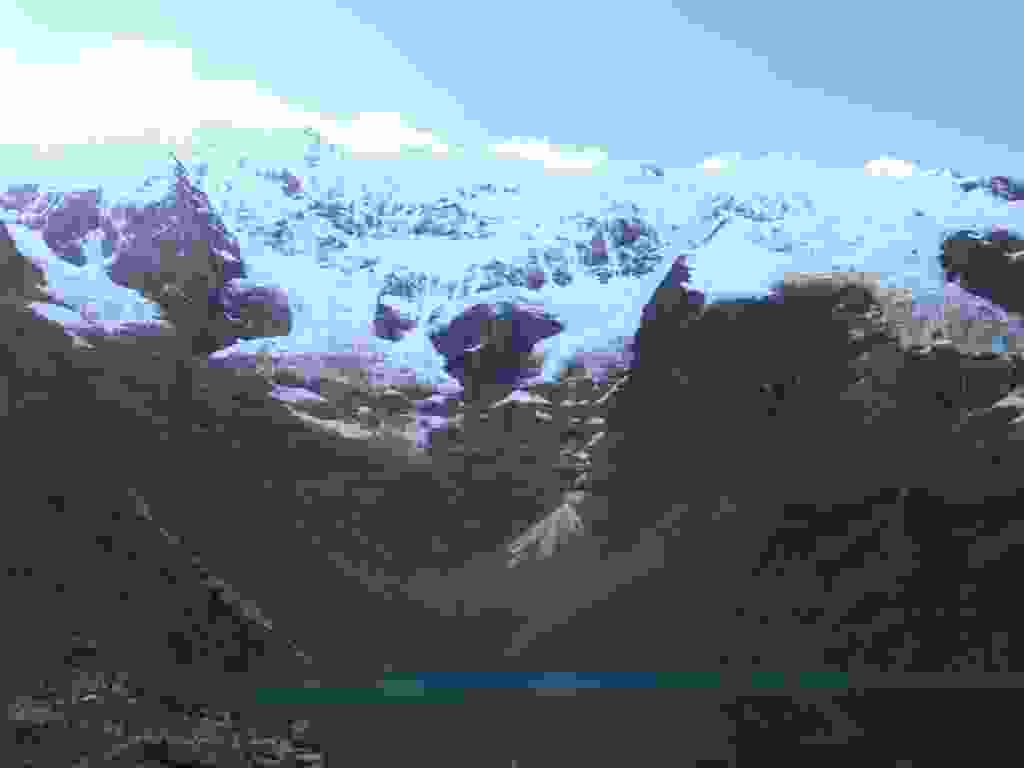
\includegraphics[width=\mywidth]{../wp-content/uploads/2015/05/P5234362-1024x768.jpg} \end{center}
\begin{center} 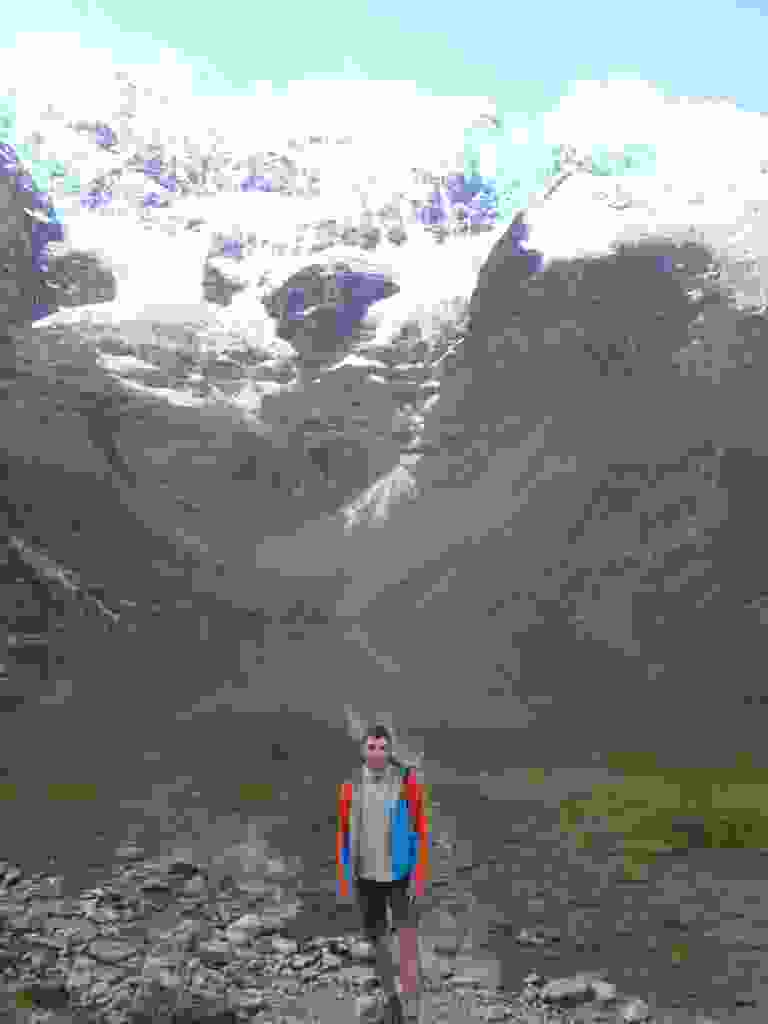
\includegraphics[width=0.58\textwidth]{../wp-content/uploads/2015/05/P5234366-768x1024.jpg} \end{center}

\subsection*{Jour 2}
Lever à 5h et grosse montée. 
\begin{center} 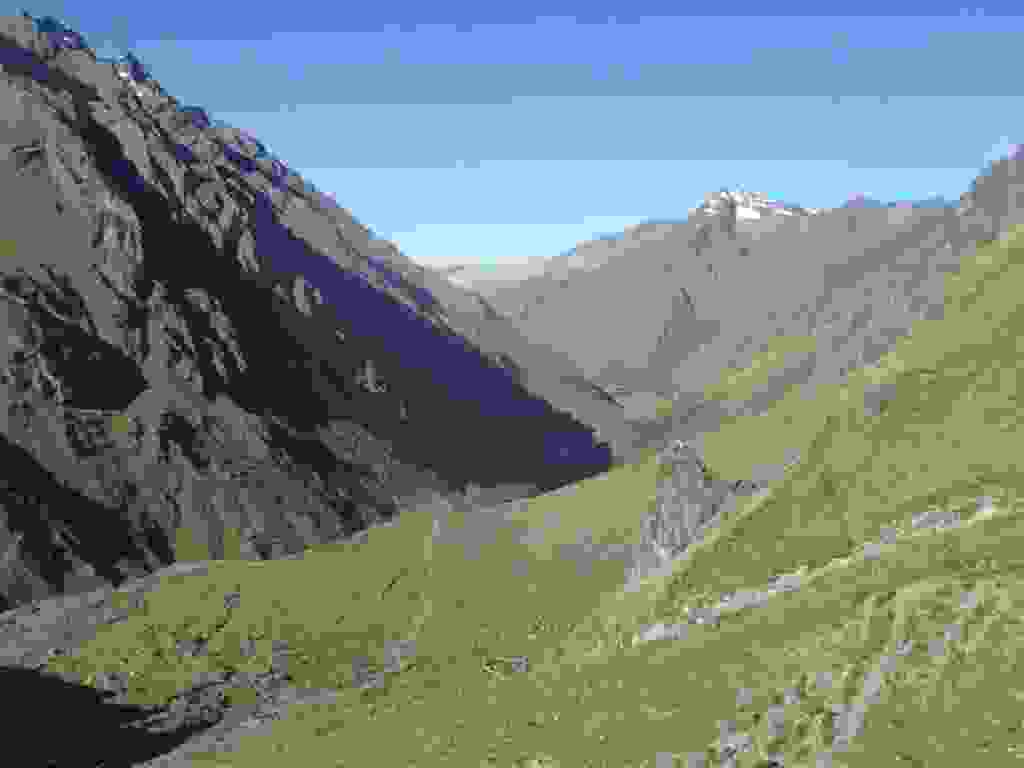
\includegraphics[width=\mywidth]{../wp-content/uploads/2015/05/P5244381-1024x768.jpg} \end{center}
\pagebreak

Le col du Salkantay à 4600m.
\begin{center} 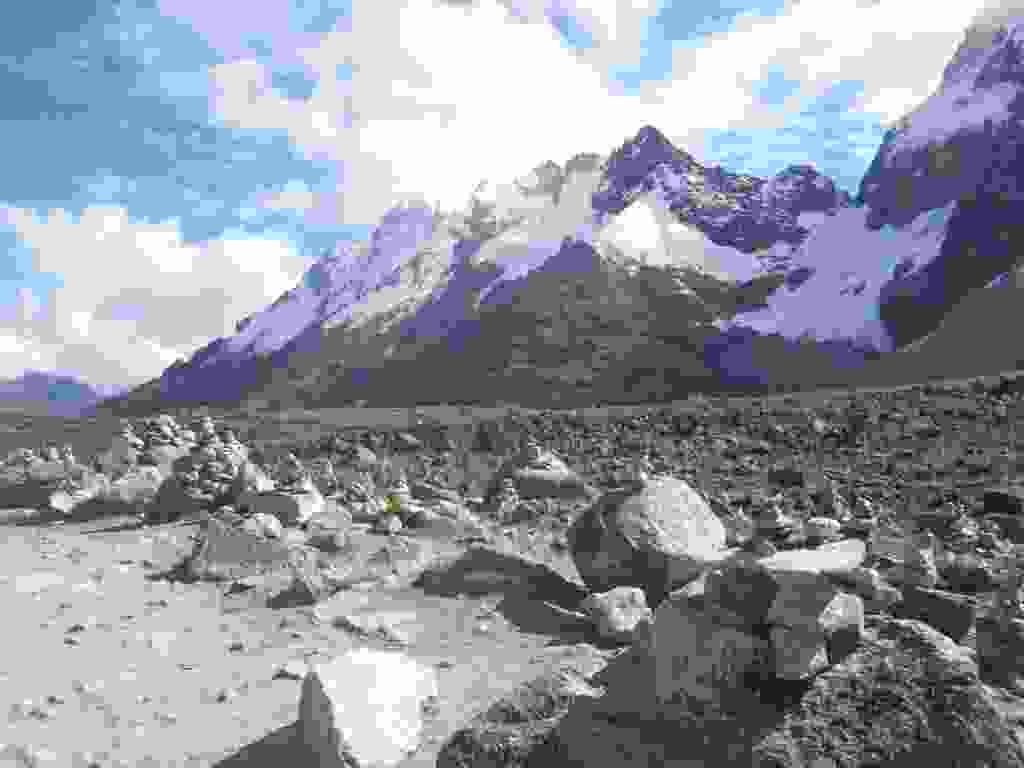
\includegraphics[width=\mywidth]{../wp-content/uploads/2015/05/P5244391-1024x768.jpg} \end{center}
~
\begin{center} 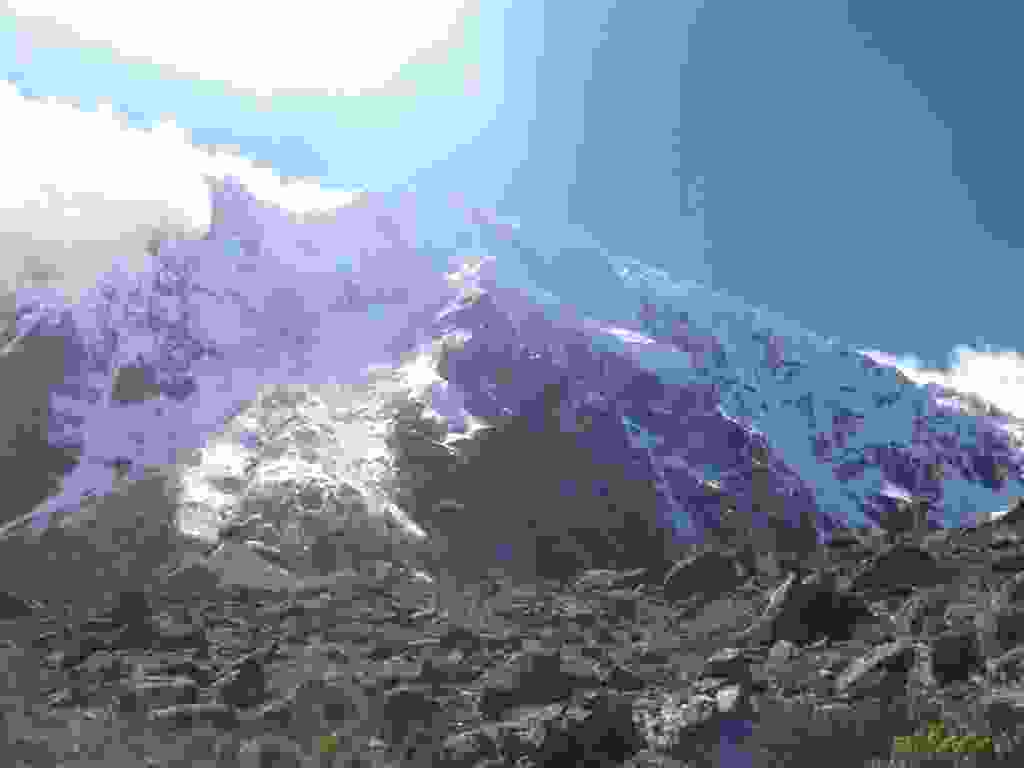
\includegraphics[width=\mywidth]{../wp-content/uploads/2015/05/P5244400-1024x768.jpg} \end{center}
\vspace{-\topsep}
\pagebreak

Le groupe au sommet avec notre guide Jean-Paul. 
\begin{center} 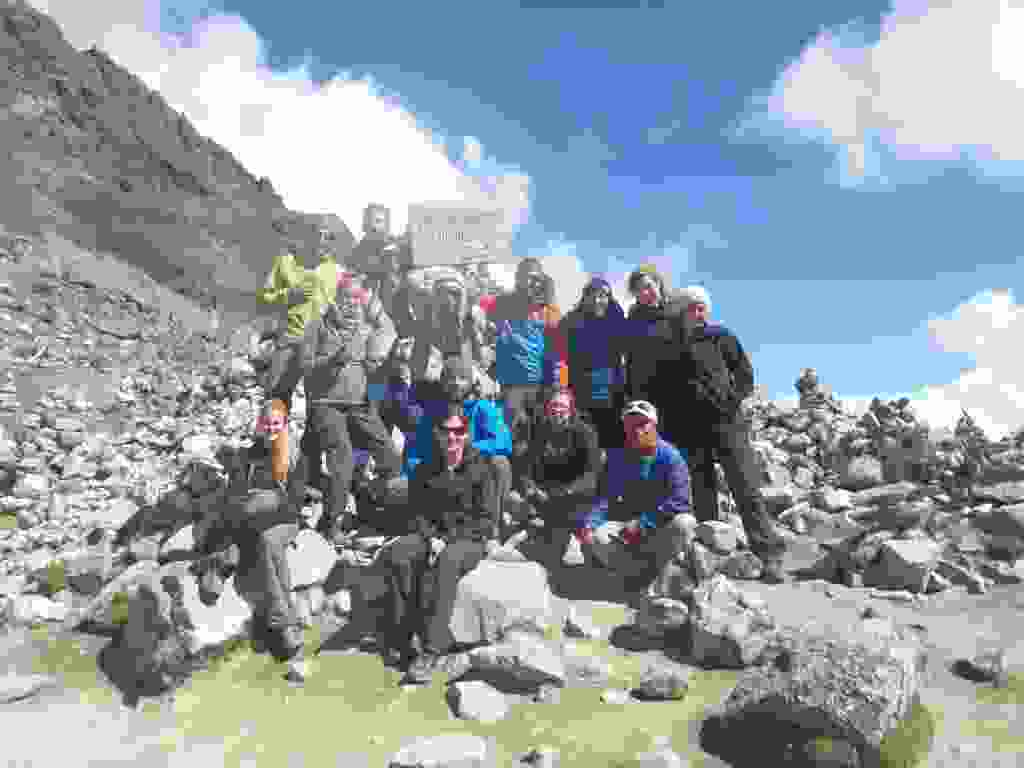
\includegraphics[width=\mywidth]{../wp-content/uploads/2015/05/P5244396-1024x768.jpg} \end{center}

La nourriture et les tentes sont portées par des chevaux. 
\begin{center} 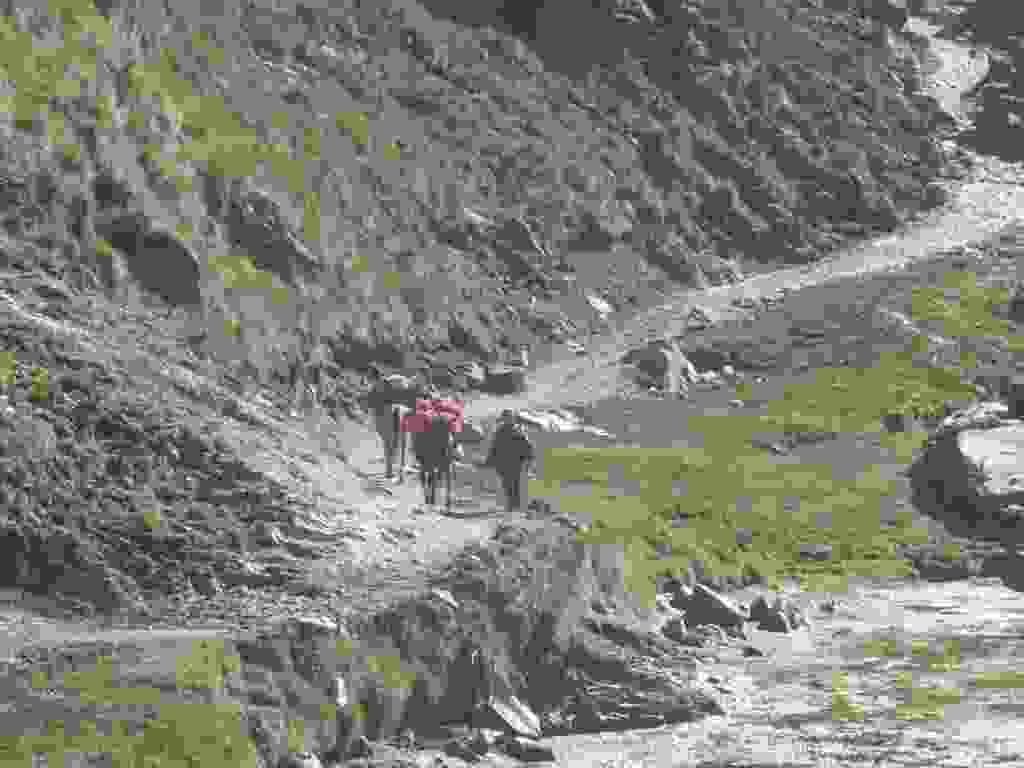
\includegraphics[width=\mywidth]{../wp-content/uploads/2015/05/P5244386-1024x768.jpg} \end{center}
\vspace{-\topsep}
\pagebreak

Longue descente jusqu'au deuxième camp à 2900m. Petit à petit on se rapproche de la jungle. 
\begin{center} 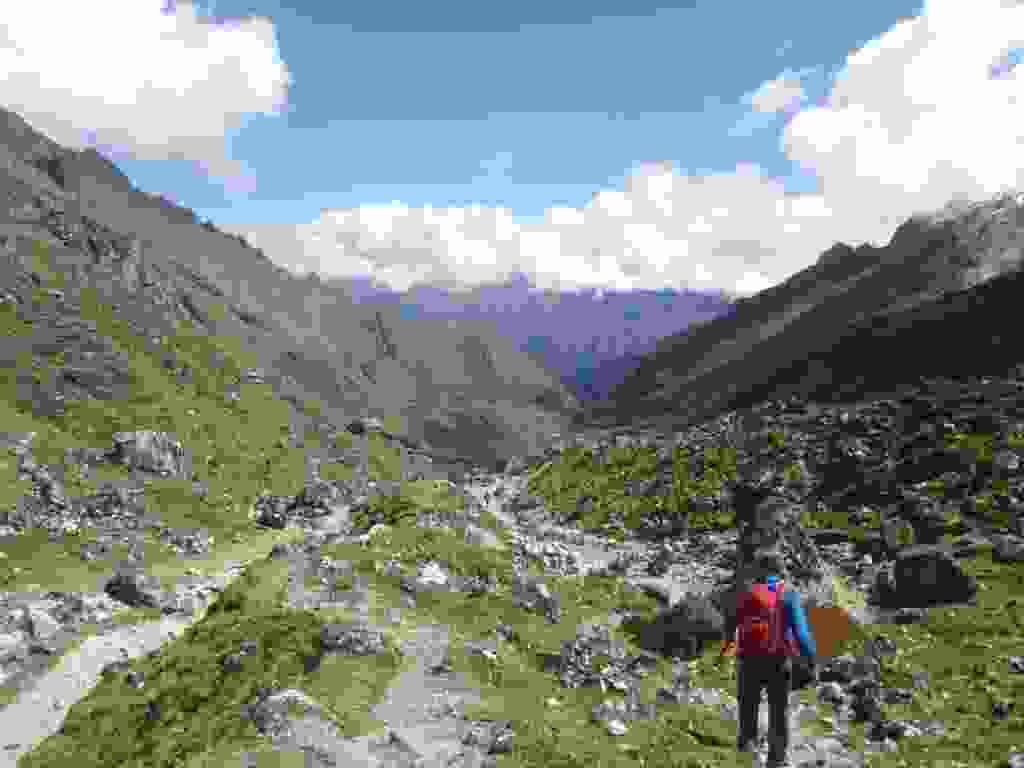
\includegraphics[width=\mywidth]{../wp-content/uploads/2015/05/P5244403-1024x768.jpg} \end{center}
\begin{center} 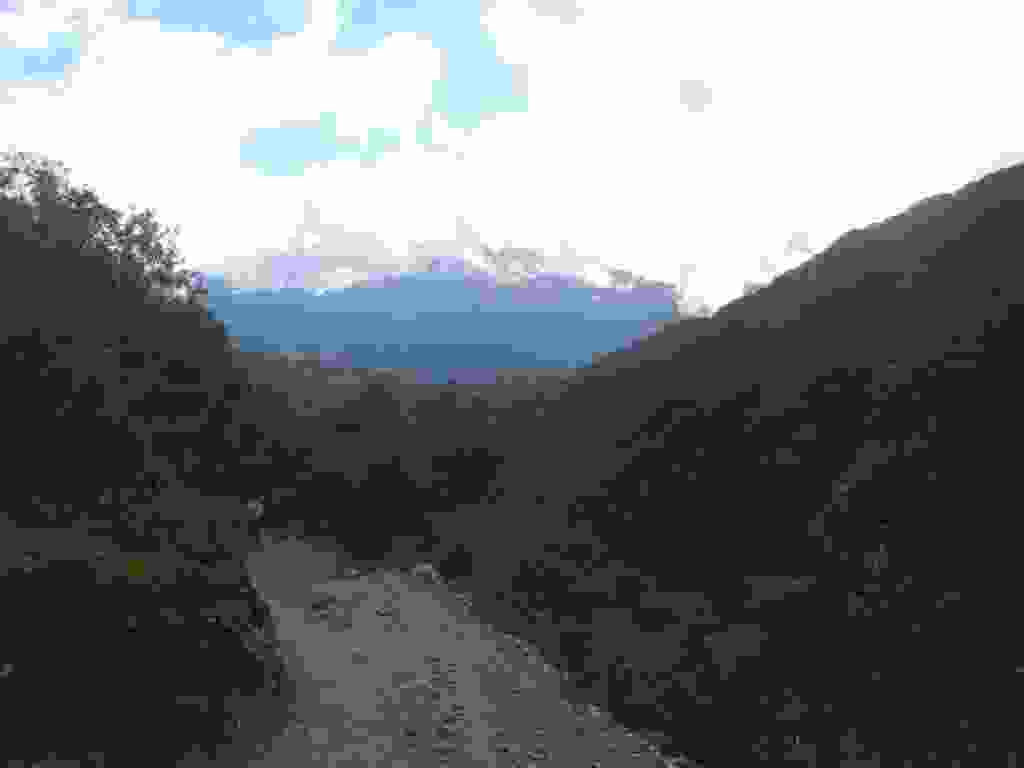
\includegraphics[width=\mywidth]{../wp-content/uploads/2015/05/P5244409-1024x768.jpg} \end{center}
\vspace{-\topsep}
\vspace{-3.25mm}
\pagebreak
~\\
\begin{center} 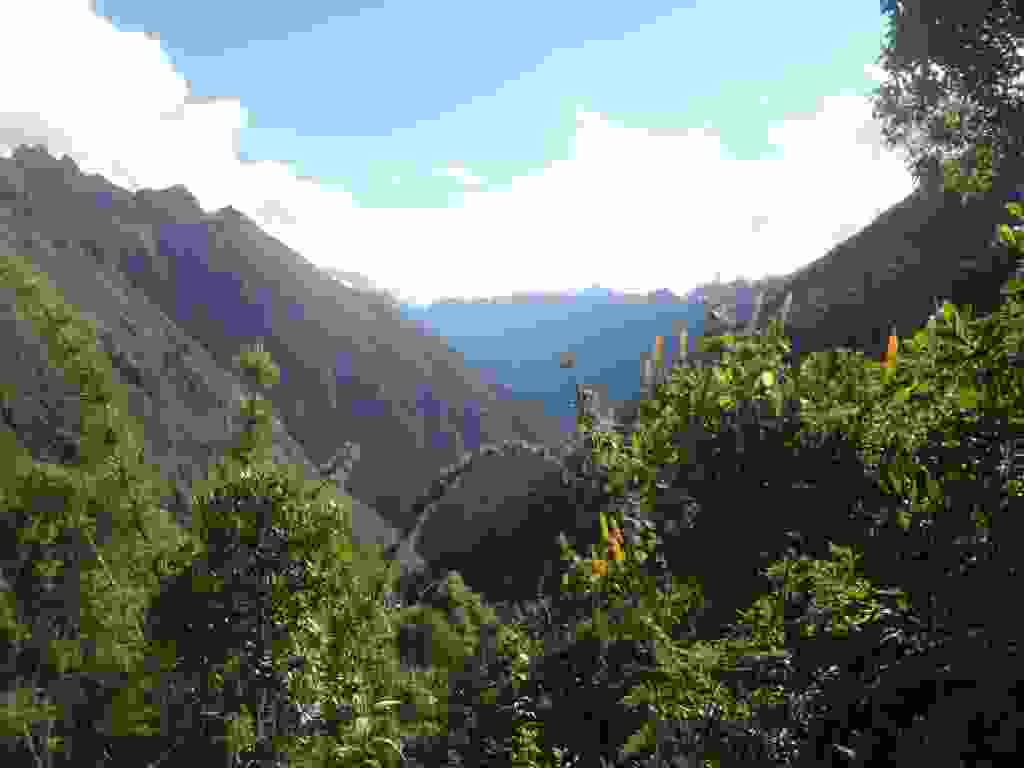
\includegraphics[width=\mywidth]{../wp-content/uploads/2015/05/P5244414-1024x768.jpg} \end{center}
\begin{center} 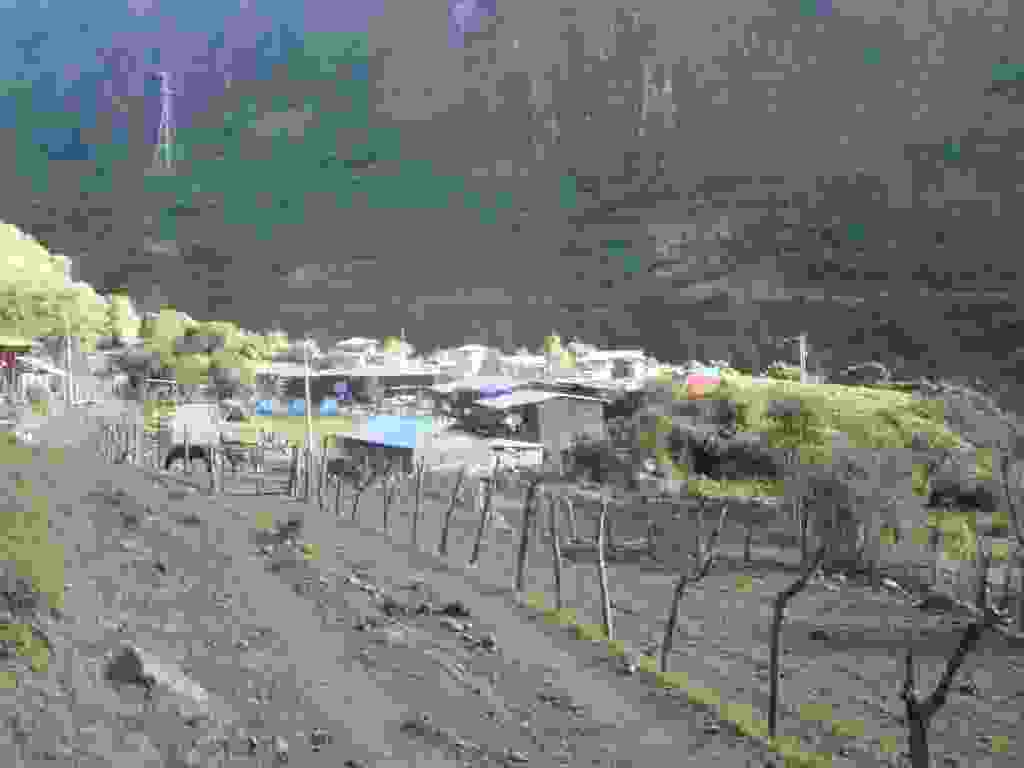
\includegraphics[width=\mywidth]{../wp-content/uploads/2015/05/P5244415-1024x768.jpg} \end{center}
\vspace{-\topsep}
\vspace{-3.25mm}
\pagebreak

\subsection*{Jour 3}
Notre groupe s'appelait \og Les Condors \fg\ pour le trek. 
\begin{center} 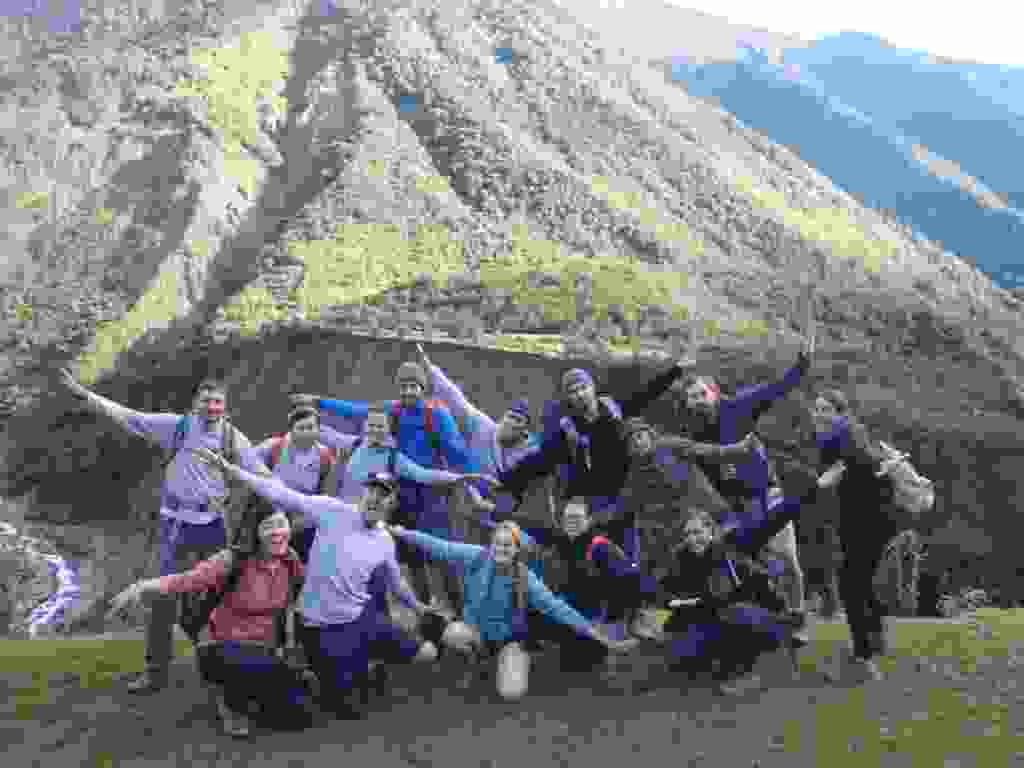
\includegraphics[width=\mywidth]{../wp-content/uploads/2015/05/P5254421-1024x768.jpg} \end{center}

On était un peu de tous les pays : France, Allemagne, Angleterre, Canada, Israël, République tchèque, ça fait parler anglais.

Le chemin alterne montées et descentes au milieu d'une végétation très dense. 
\begin{center} 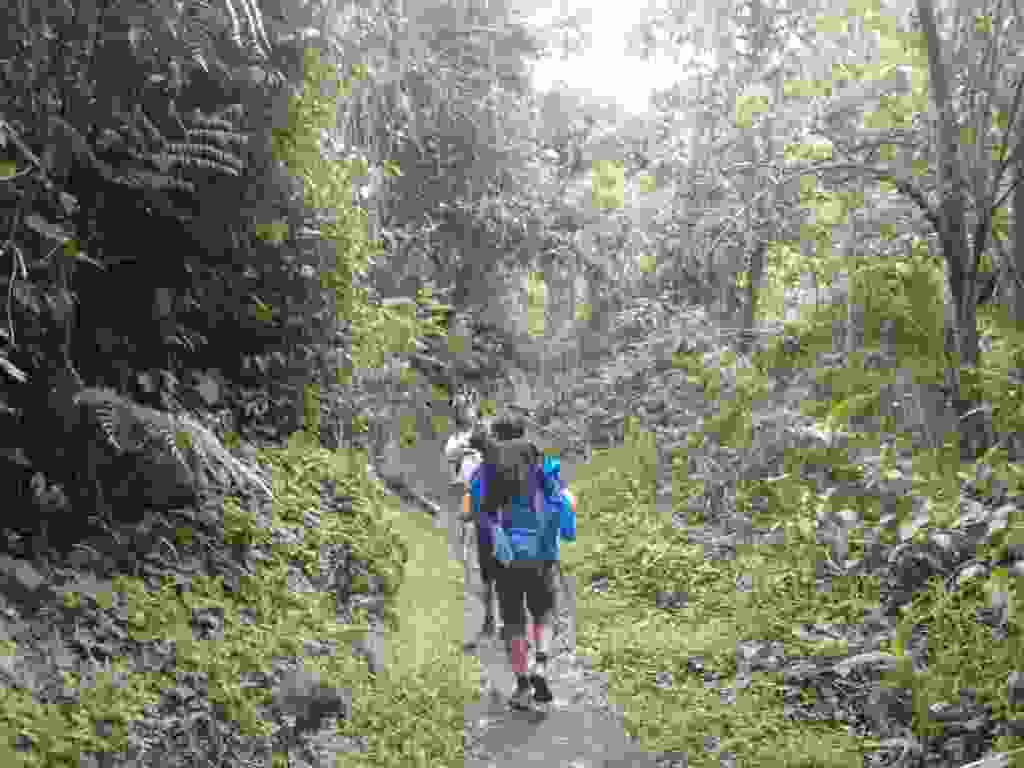
\includegraphics[width=\mywidth]{../wp-content/uploads/2015/05/P5254428-1024x768.jpg} \end{center}

\begin{center} 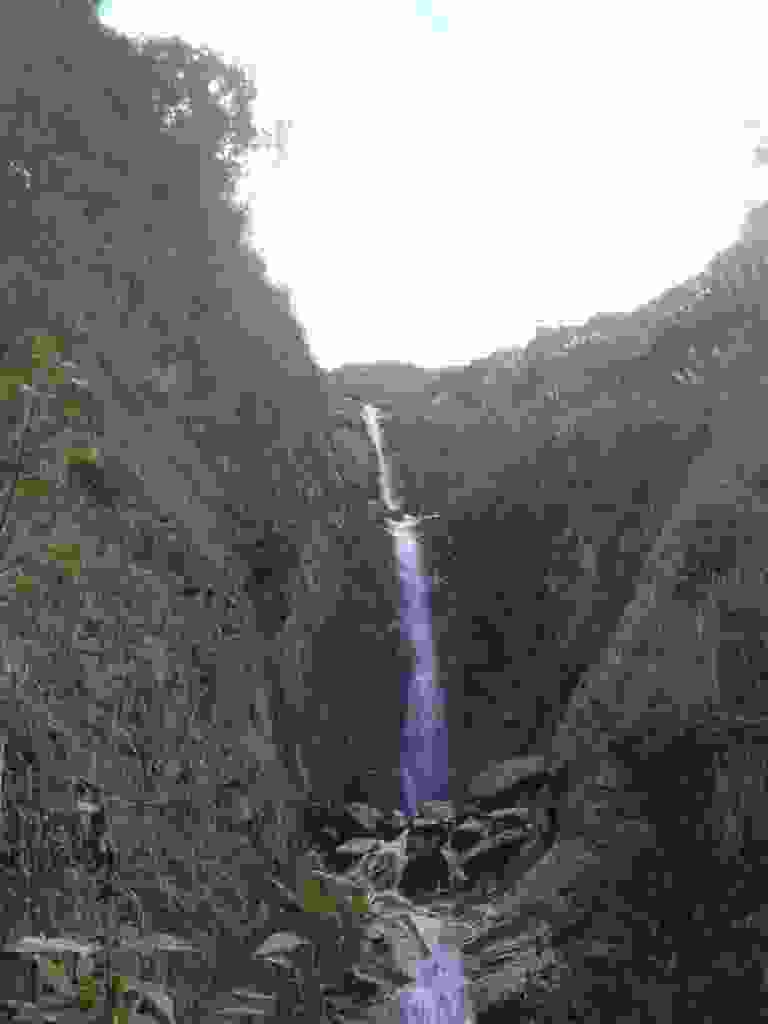
\includegraphics[width=0.6\textwidth]{../wp-content/uploads/2015/05/P5254424-768x1024.jpg} \end{center}

On croise quelques arbres fruitiers. 
\begin{center} 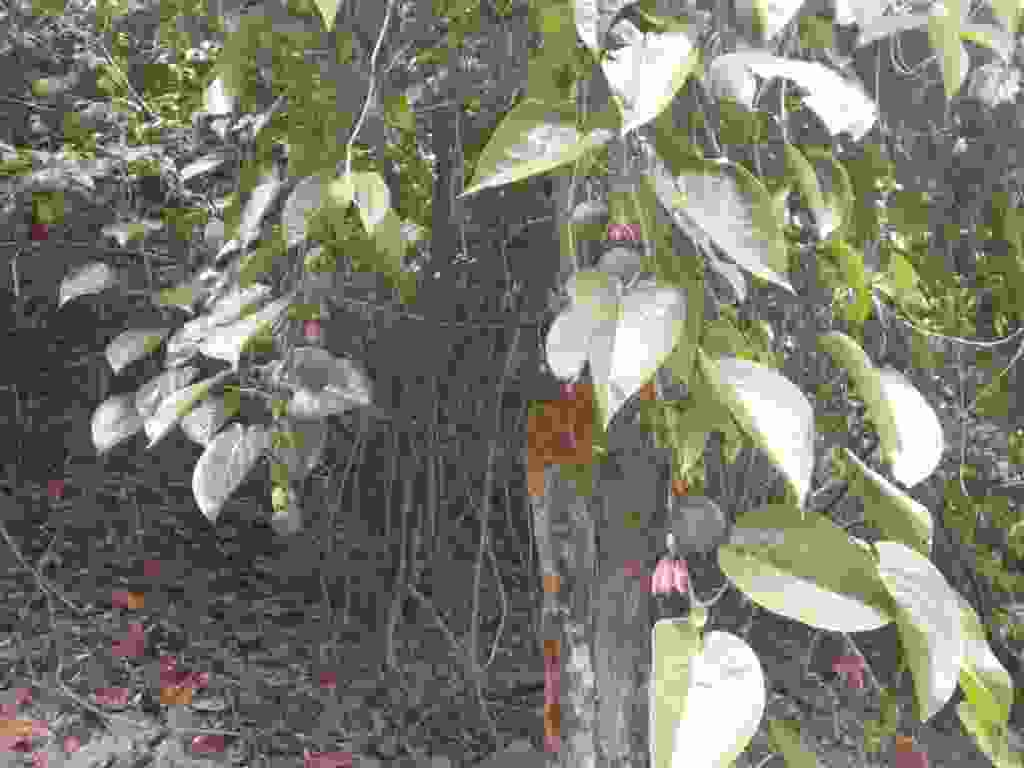
\includegraphics[width=\mywidth]{../wp-content/uploads/2015/05/P5254427-1024x768.jpg} \end{center}
\vspace{-\topsep}
\pagebreak
~\\
\begin{center} 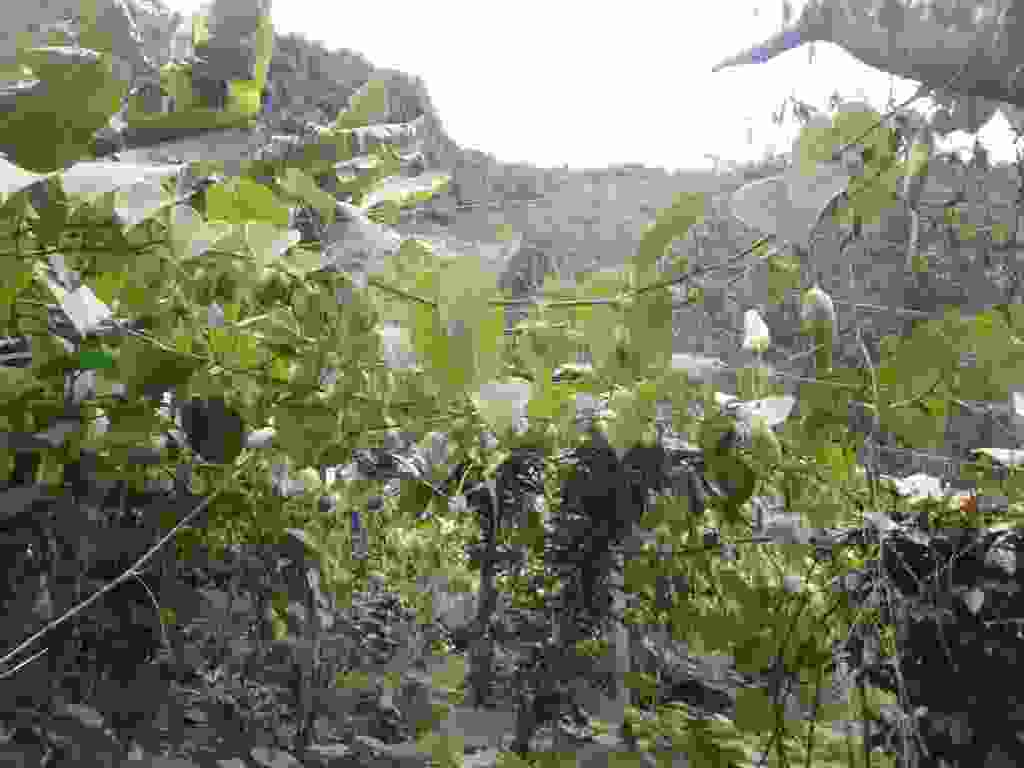
\includegraphics[width=\mywidth]{../wp-content/uploads/2015/05/P5254430-1024x768.jpg} \end{center}
~
\begin{center} 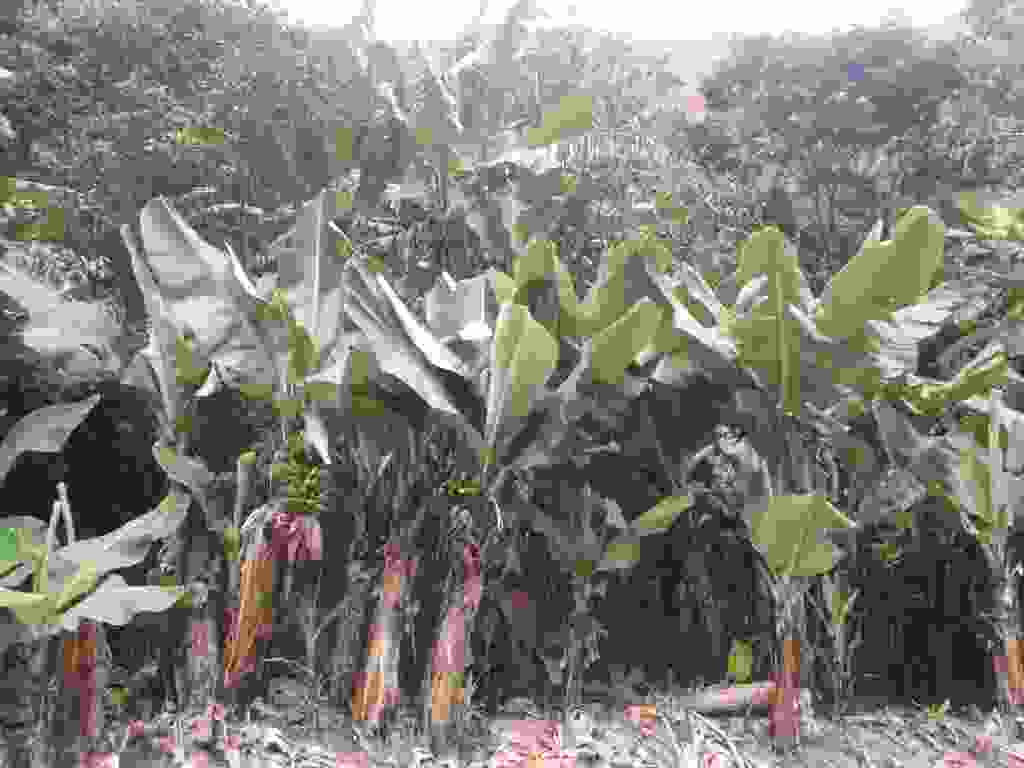
\includegraphics[width=\mywidth]{../wp-content/uploads/2015/05/P5264440-1024x768.jpg} \end{center}
\vspace{-\topsep}
\pagebreak

Repas de midi à Santa Maria : le cuisiner du trek nous gâte avec des spécialités péruviennes, ceviche et papas rellenas. 
\begin{center} 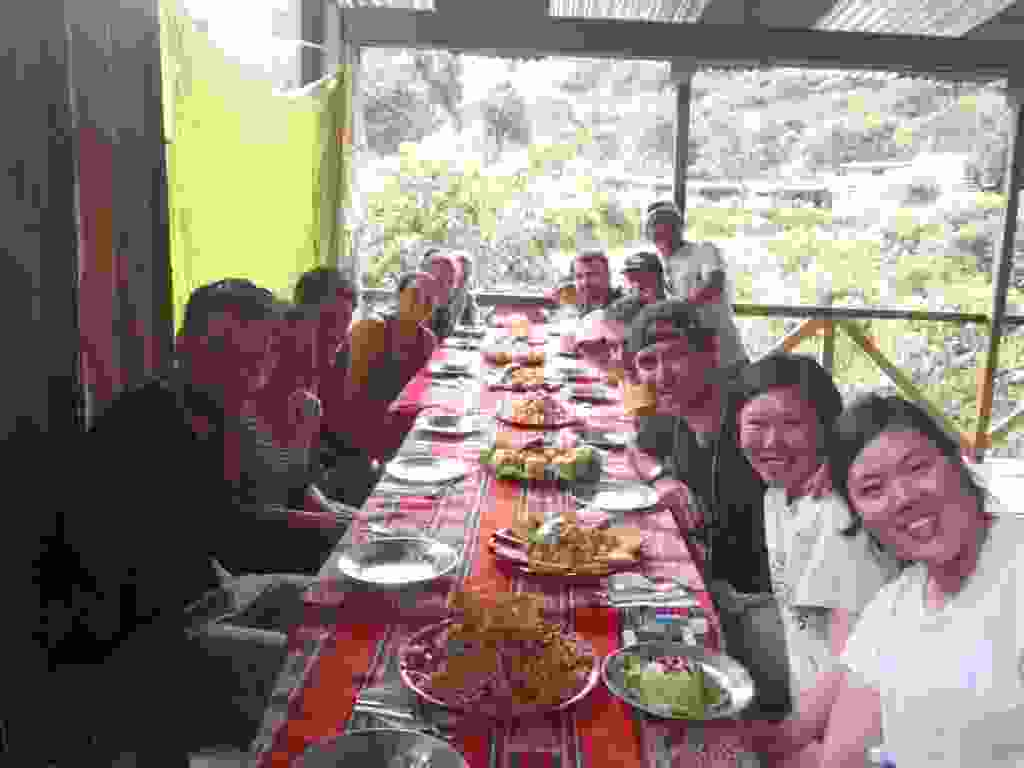
\includegraphics[width=\mywidth]{../wp-content/uploads/2015/05/P5254431-1024x768.jpg} \end{center}

Un bon moment aux bains de Santa Teresa. 
\begin{center} 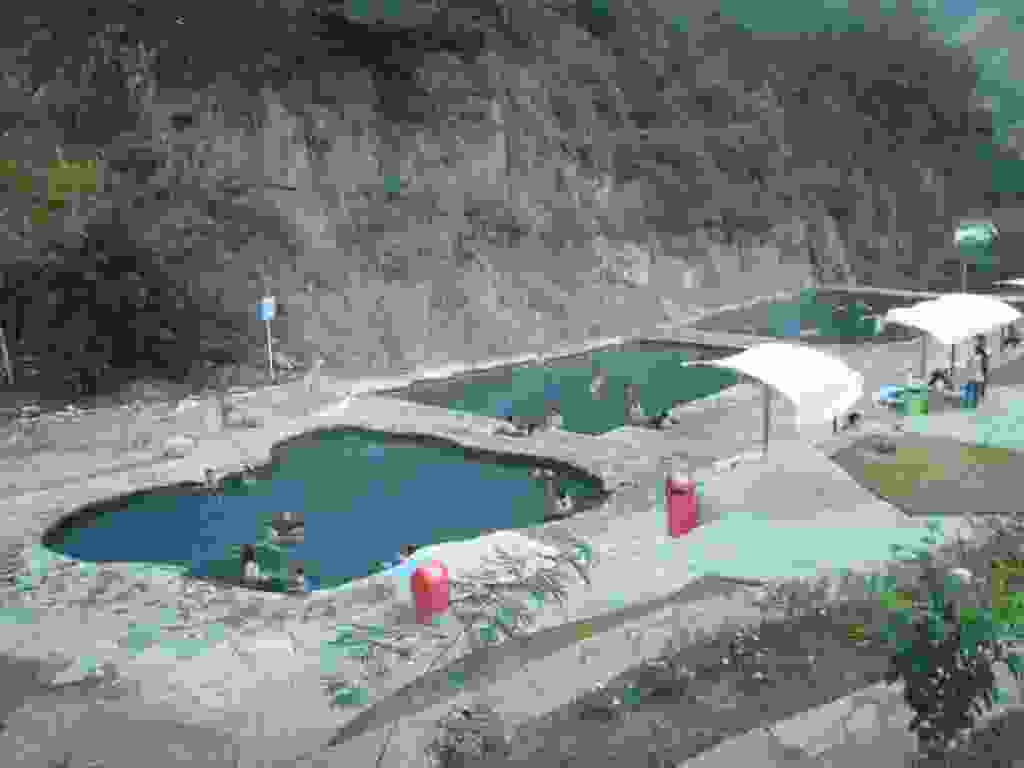
\includegraphics[width=\mywidth]{../wp-content/uploads/2015/05/P5264435-1024x768.jpg} \end{center}
\vspace{-\topsep}
\pagebreak

\subsection*{Jour 4} 
Le matin marche sur la route pour arriver à Hidroelectrica. 
\begin{center} 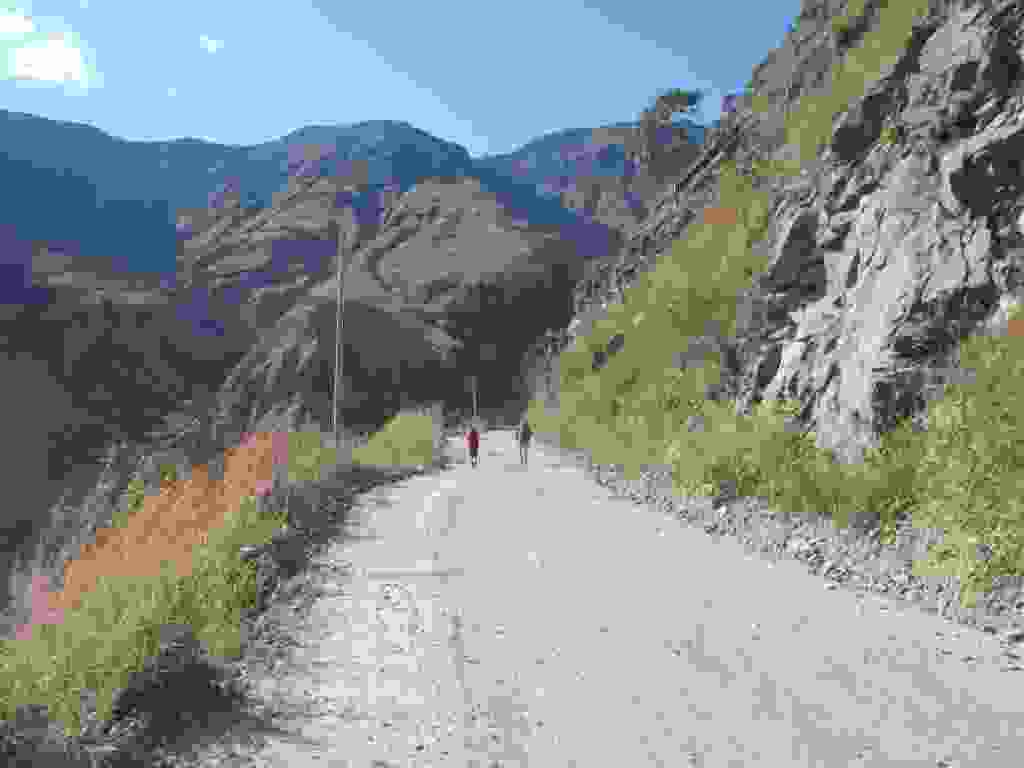
\includegraphics[width=\mywidth]{../wp-content/uploads/2015/05/P5264437-1024x768.jpg} \end{center}

L'après-midi, le long de la voie ferrée jusqu'au village en bas du Machu Picchu : Aguas Calientes. 
\begin{center} 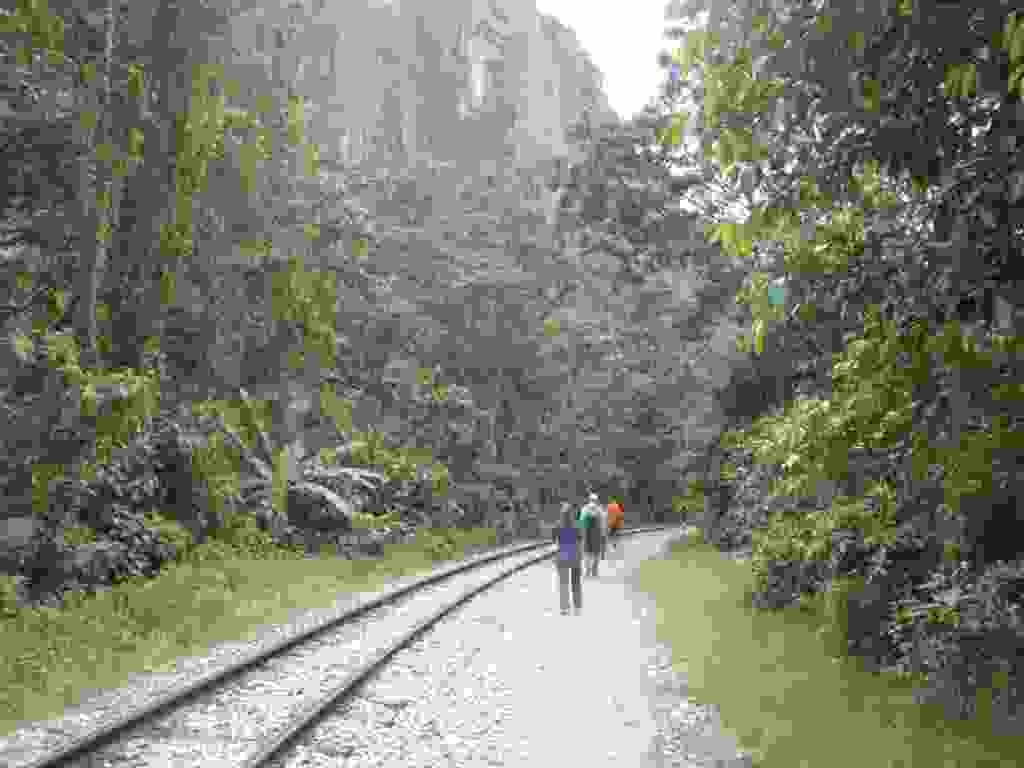
\includegraphics[width=\mywidth]{../wp-content/uploads/2015/05/P5264442-1024x768.jpg} \end{center}
\begin{center} 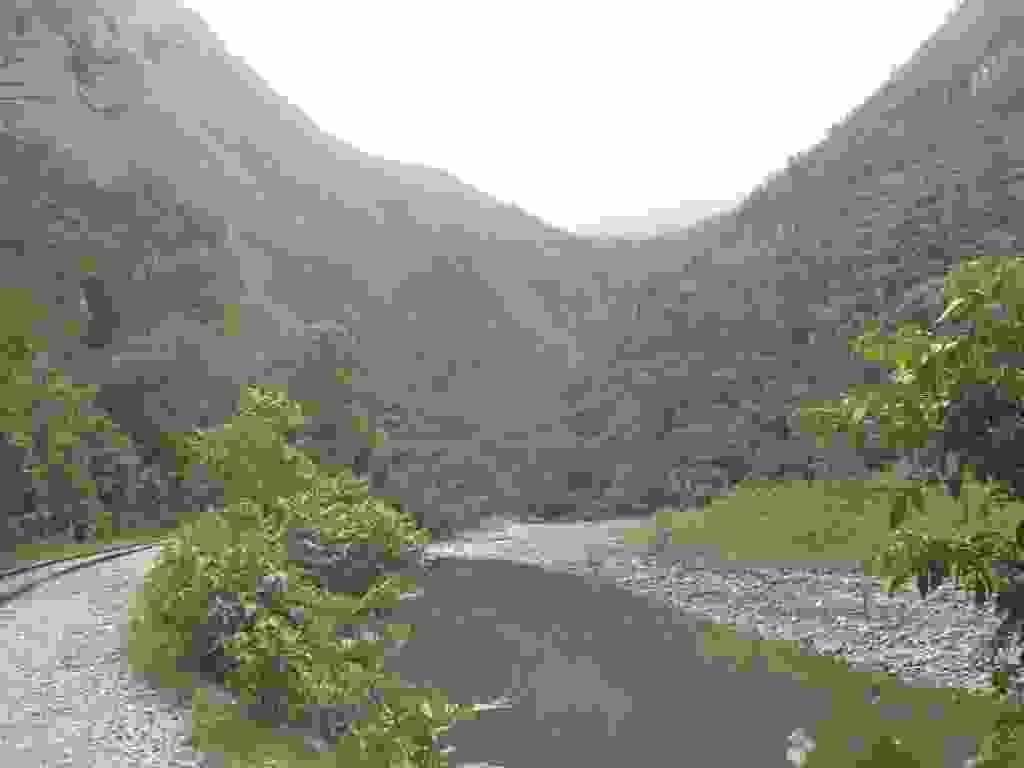
\includegraphics[width=\mywidth]{../wp-content/uploads/2015/05/P5264444-1024x768.jpg} \end{center}

Ce village n'est accessible qu'en train ou à pied, on y trouve quasiment que des hôtels et des restaurants où les prix sont multipliés par 3 ou 4 par rapport au reste du Pérou. 
\begin{center} 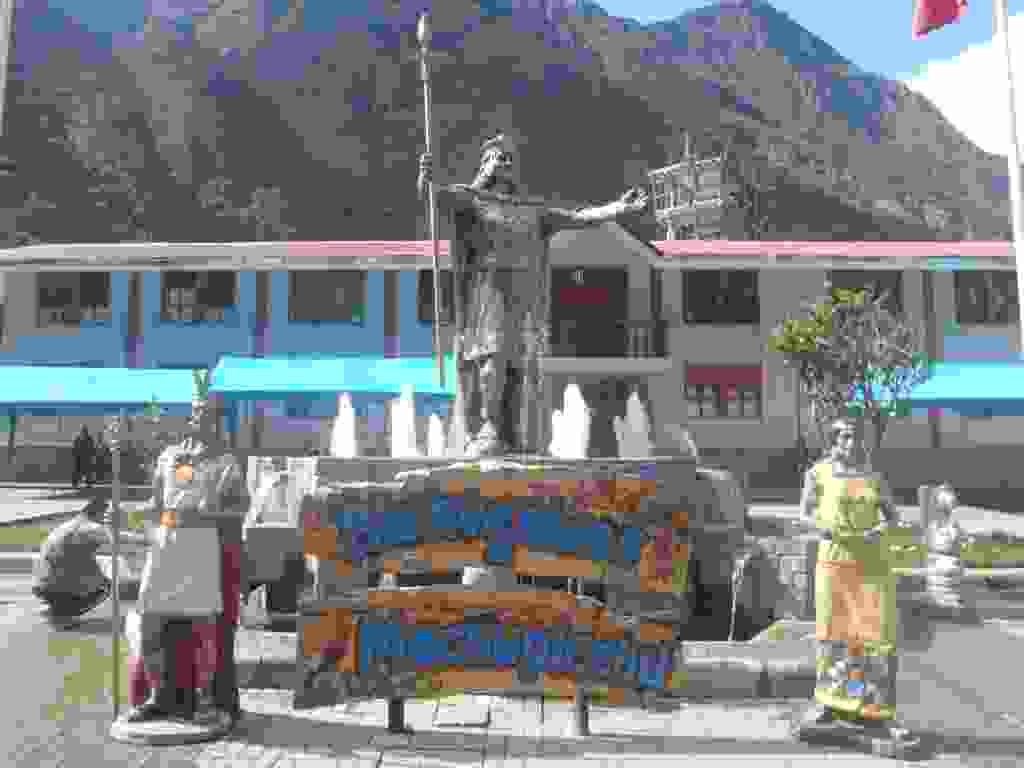
\includegraphics[width=\mywidth]{../wp-content/uploads/2015/06/P5284557-1024x768.jpg} \end{center}
\begin{center} 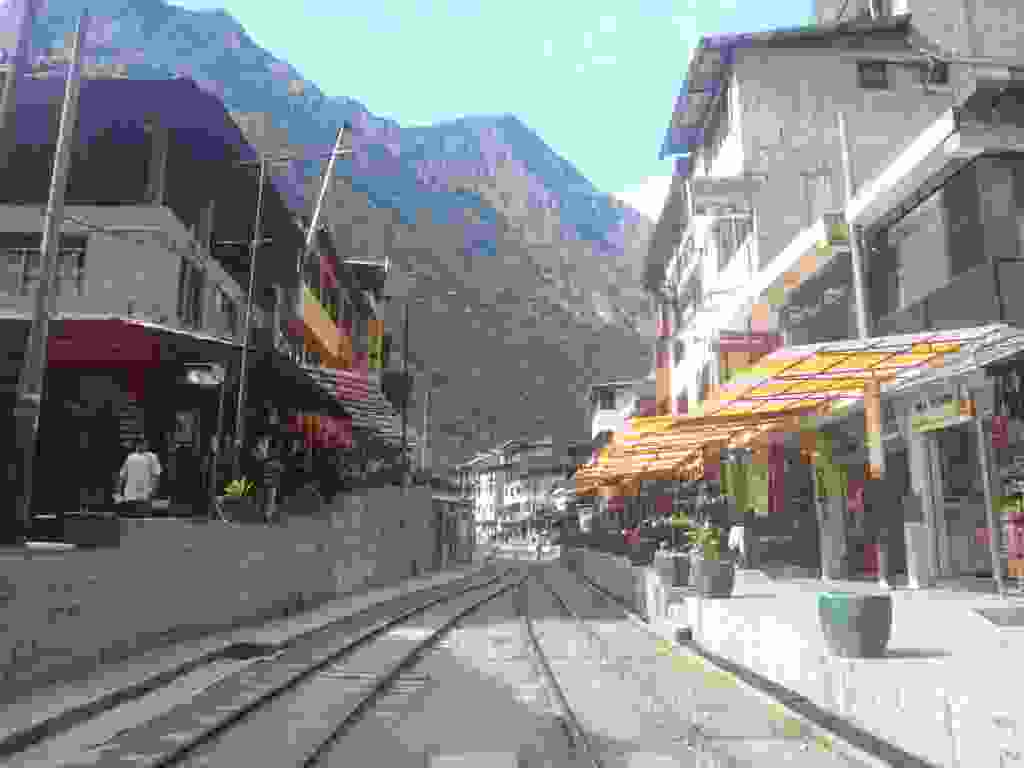
\includegraphics[width=\mywidth]{../wp-content/uploads/2015/06/P5284560-1024x768.jpg} \end{center}

\subsection*{Jour 5} 
Départ à 4h30 pour arriver au premier point de contrôle du Machu Picchu avant l'ouverture à 5h.  1h de montée à la frontale jusqu'à l'entrée du Machu Picchu qui ouvre à 6h. 
Premières photos du Machu Picchu encore presque désert à cette heure là. 
\begin{center} 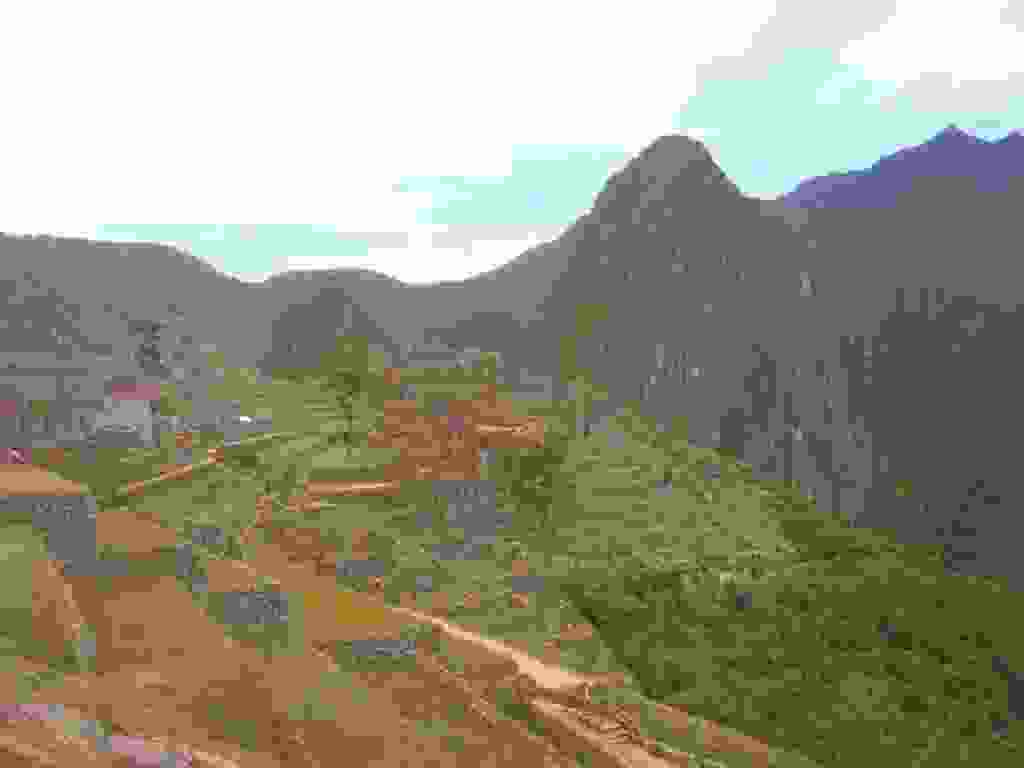
\includegraphics[width=\mywidth]{../wp-content/uploads/2015/06/P5274452-1024x768.jpg} \end{center}
\begin{center} 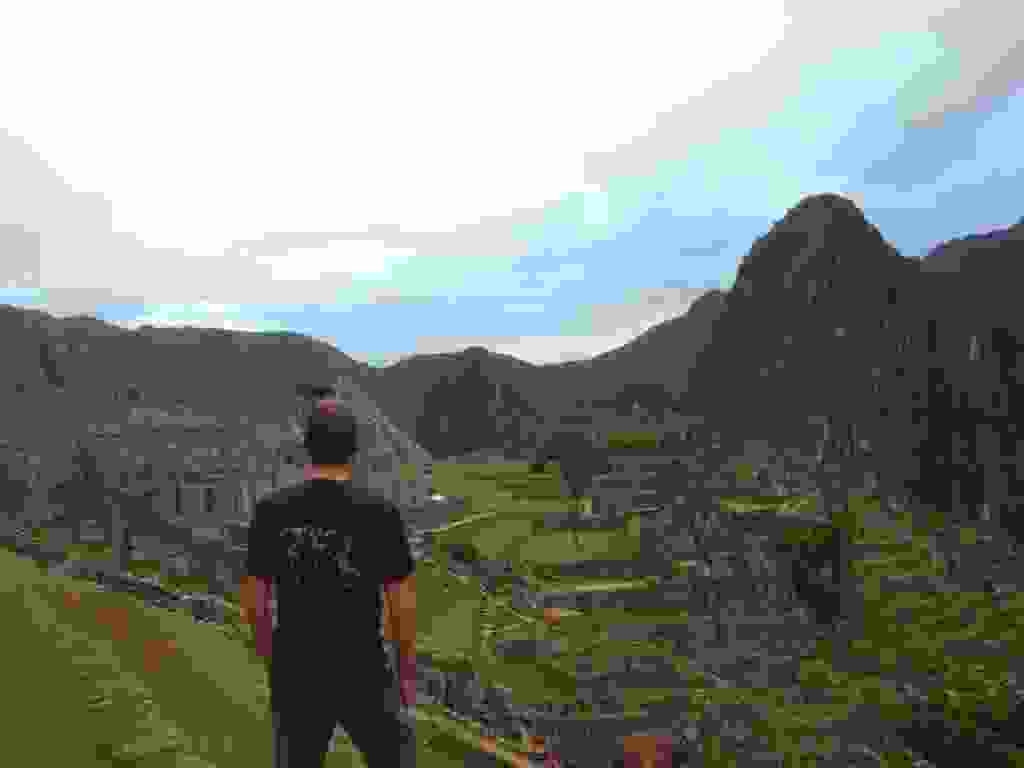
\includegraphics[width=\mywidth]{../wp-content/uploads/2015/06/P5274457-1024x768.jpg} \end{center}

Le lever du soleil sur les montagnes. 
\begin{center} 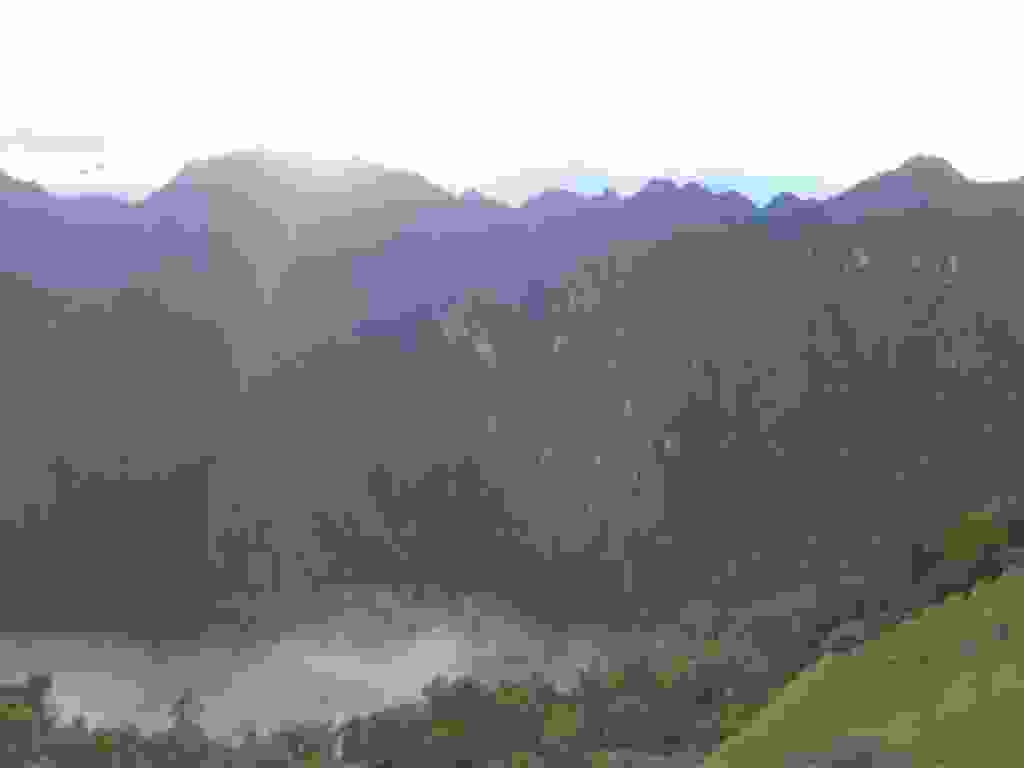
\includegraphics[width=\mywidth]{../wp-content/uploads/2015/06/P5274465-1024x768.jpg} \end{center}
\vspace{-\topsep}
\pagebreak

Petite visite guidée pour voir quelques endroits intéressants.
\begin{center} 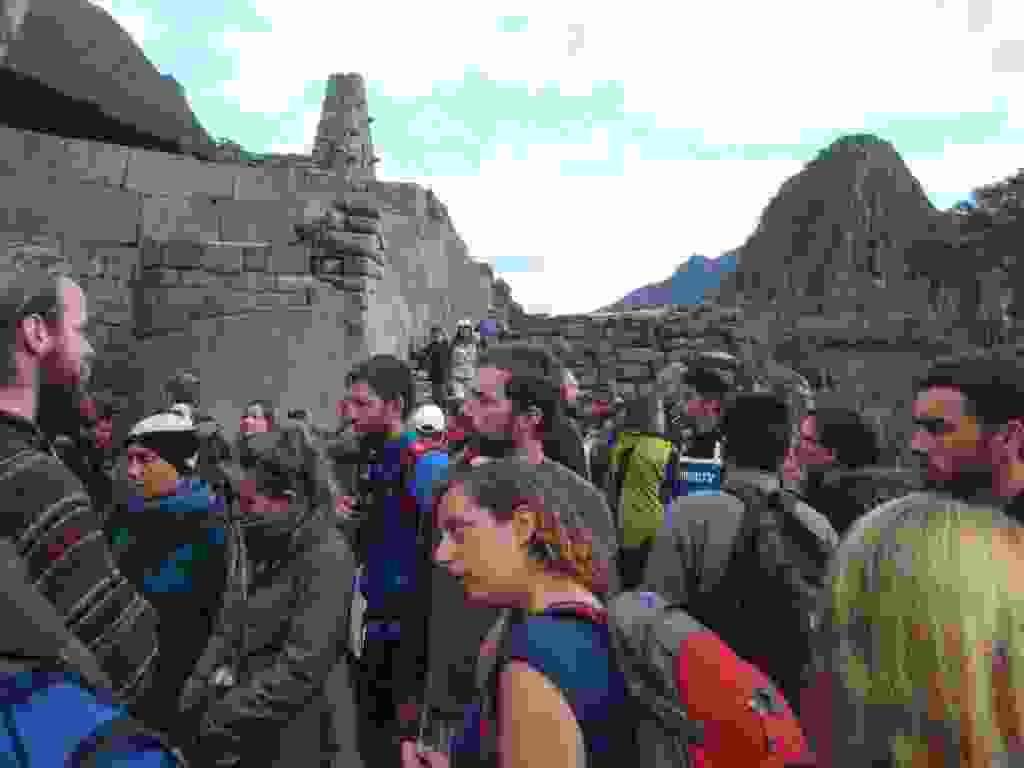
\includegraphics[width=\mywidth]{../wp-content/uploads/2015/06/P5274466-1024x768.jpg} \end{center}

Le temple du soleil. 
\begin{center} 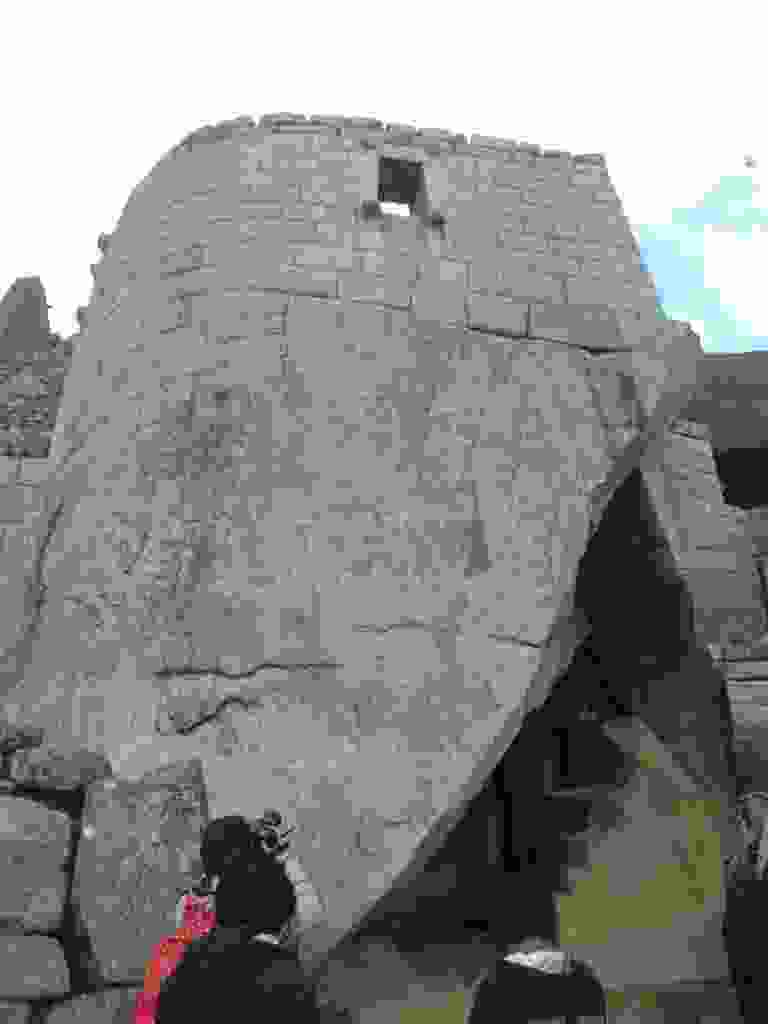
\includegraphics[height=0.82\textwidth]{../wp-content/uploads/2015/06/P5274464-768x1024.jpg} \end{center}
\vspace{-\topsep}
\pagebreak
~
\vspace{-11mm}
\begin{center} 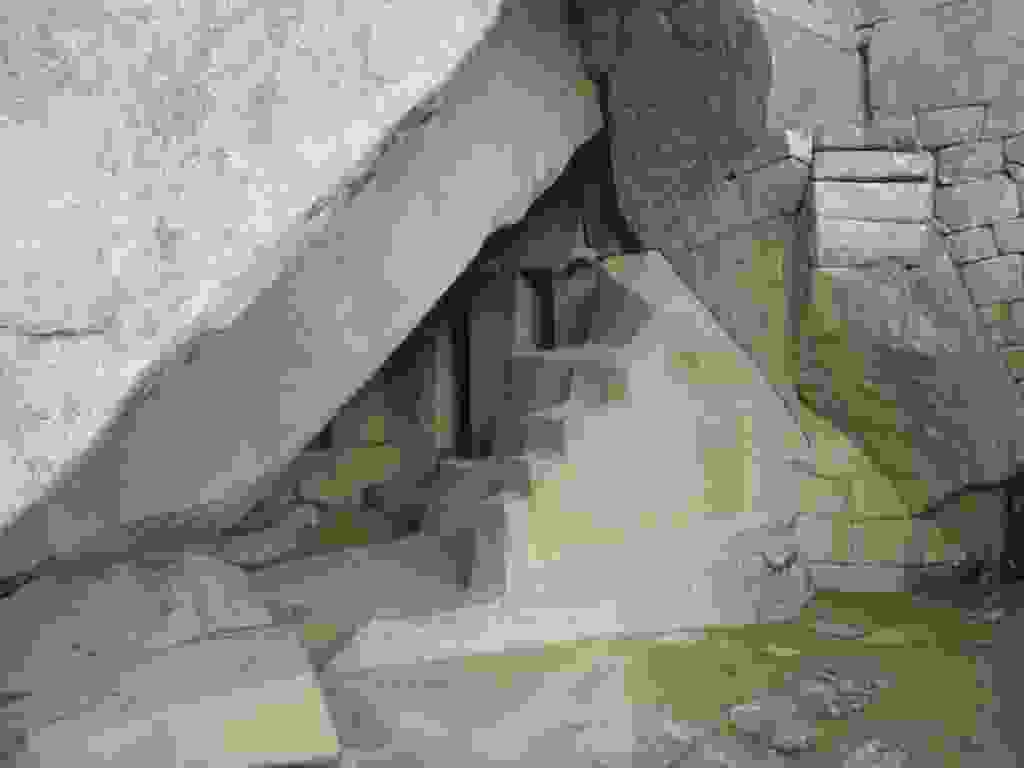
\includegraphics[width=\mywidth]{../wp-content/uploads/2015/06/P5274462-1024x768.jpg} \end{center}

Les miroirs d'eau. 
\begin{center} 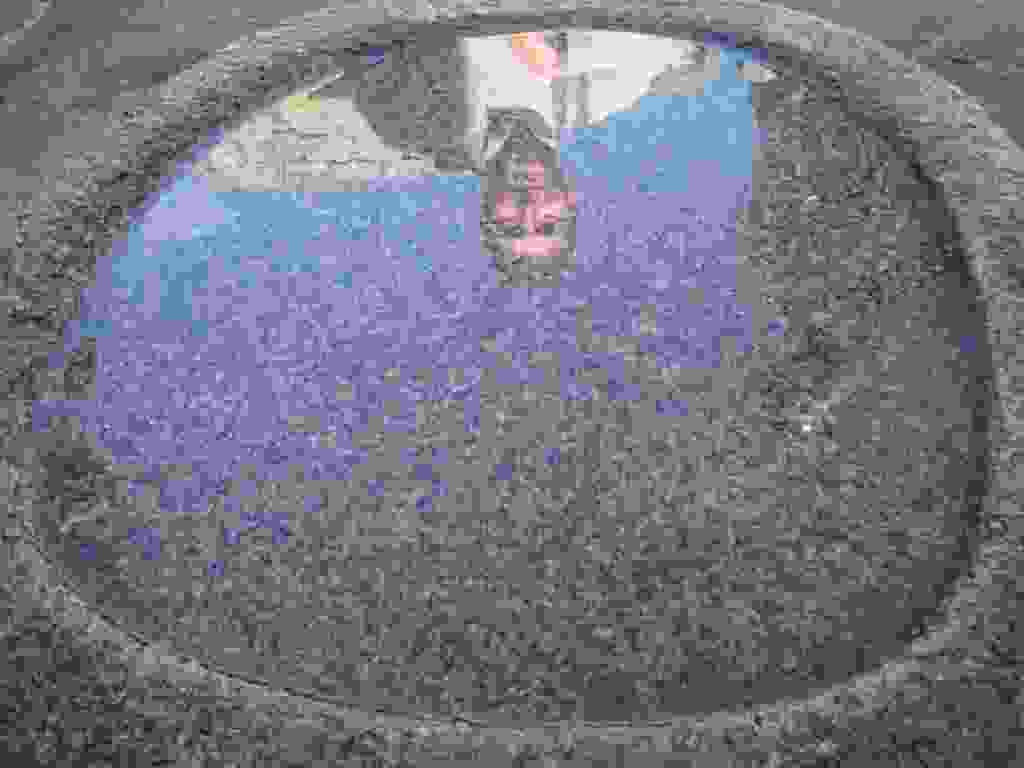
\includegraphics[width=\mywidth]{../wp-content/uploads/2015/06/P5274487-1024x768.jpg} \end{center}
\vspace{-\topsep}
\pagebreak

Temple des 3 fenêtres. 
\begin{center} 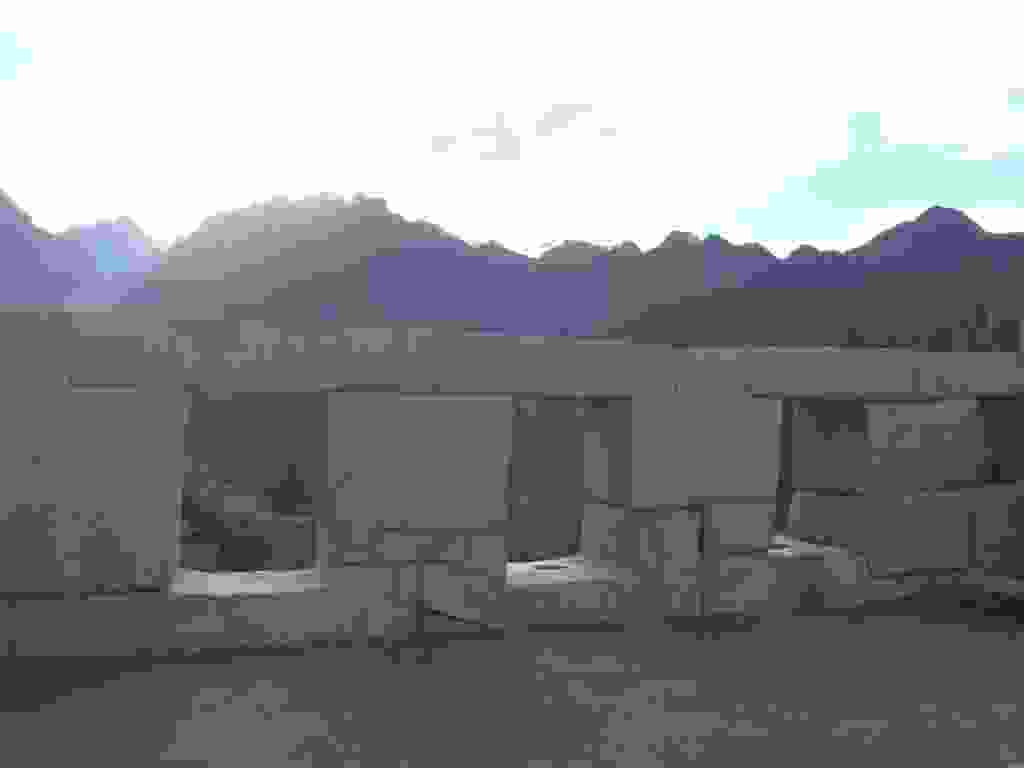
\includegraphics[width=\mywidth]{../wp-content/uploads/2015/06/P5274480-1024x768.jpg} \end{center}

Temple principal. 
\begin{center} 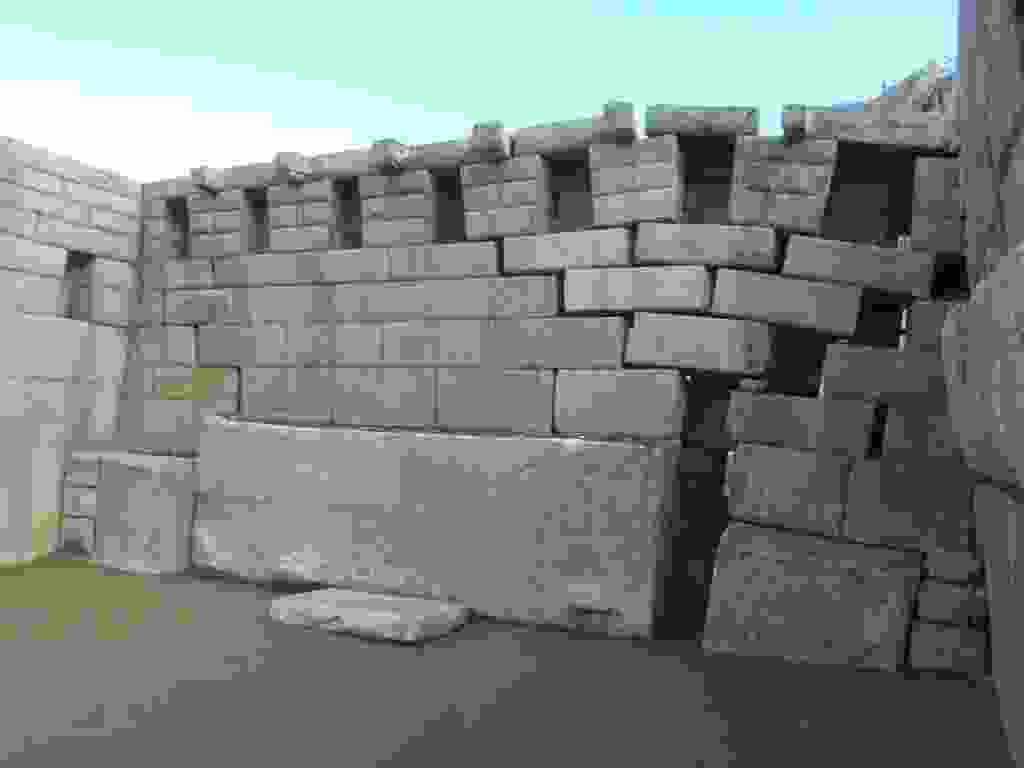
\includegraphics[width=\mywidth]{../wp-content/uploads/2015/06/P5274478-1024x768.jpg} \end{center}
\vspace{-\topsep}
\pagebreak

Des murs incas parasismiques : du bon boulot. 
\begin{center} 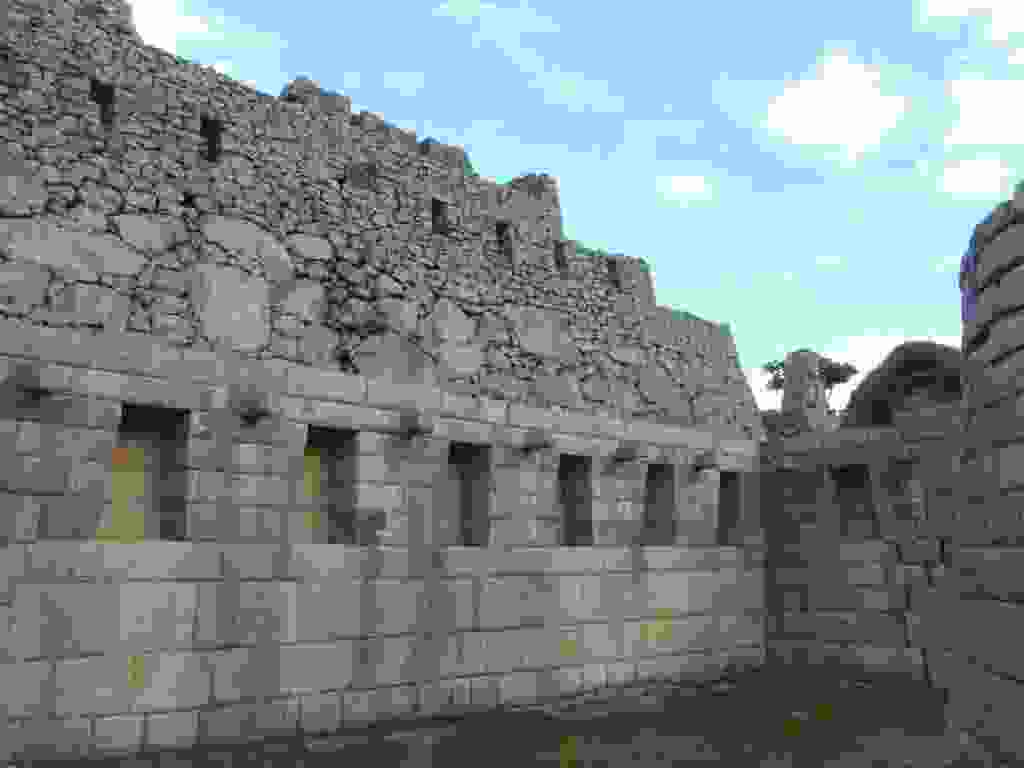
\includegraphics[width=\mywidth]{../wp-content/uploads/2015/06/P5274468-1024x768.jpg} \end{center}
~
\begin{center} 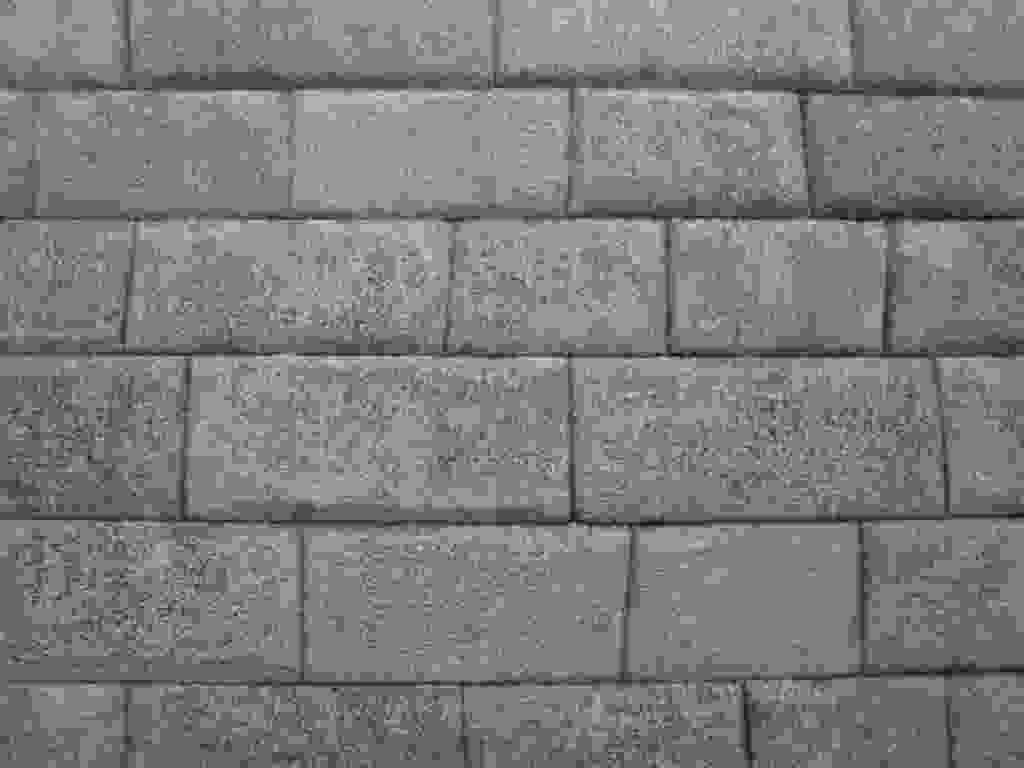
\includegraphics[width=\mywidth]{../wp-content/uploads/2015/06/P5274469-1024x768.jpg} \end{center}
\vspace{-\topsep}
\pagebreak

Un petit tour du site.
\begin{center} 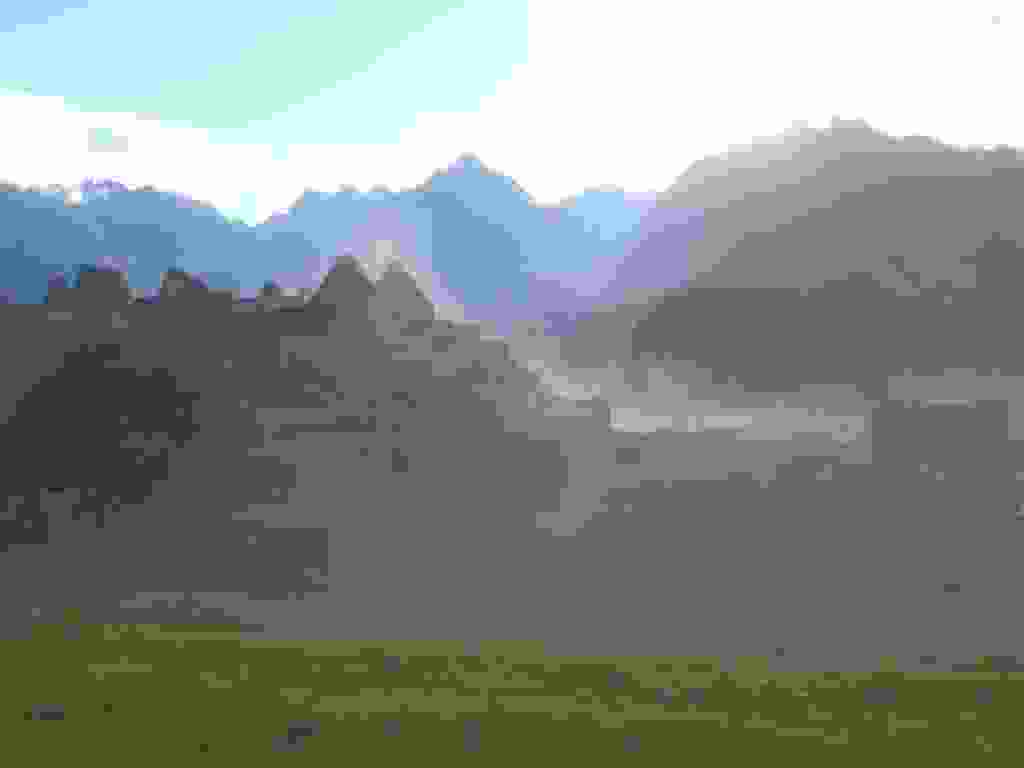
\includegraphics[width=\mywidth]{../wp-content/uploads/2015/06/P5274483-1024x768.jpg} \end{center}
\begin{center} 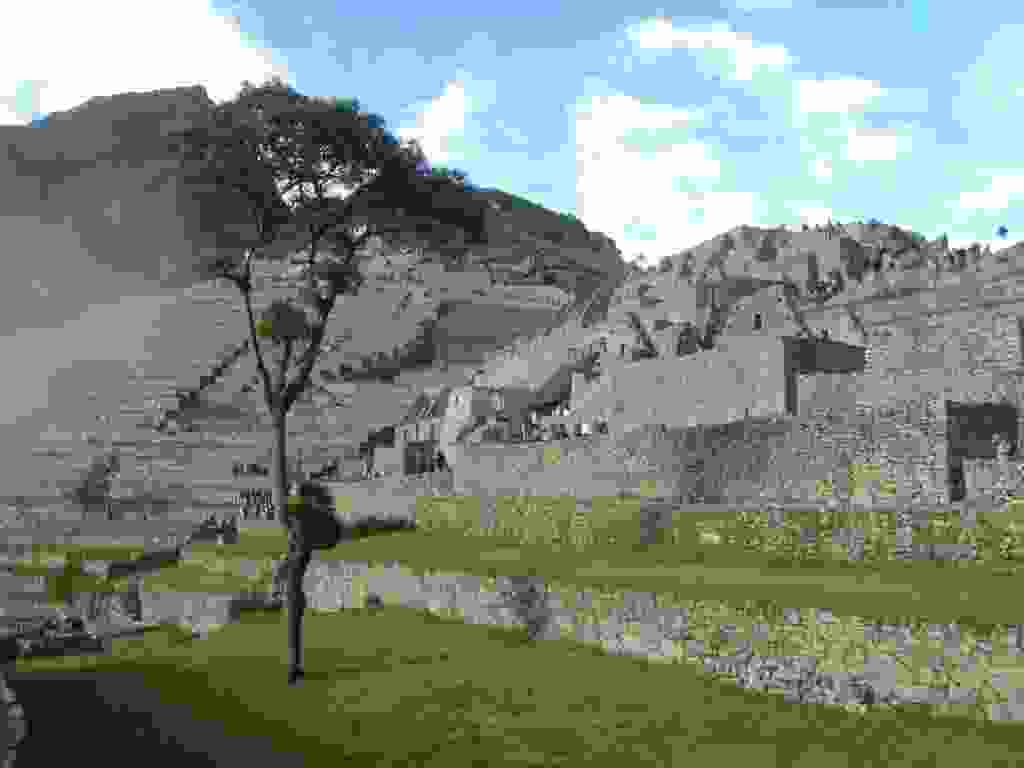
\includegraphics[width=\mywidth]{../wp-content/uploads/2015/06/P5274484-1024x768.jpg} \end{center}
\vspace{-\topsep}
\vspace{-3.25mm}
\pagebreak
~
\begin{center} 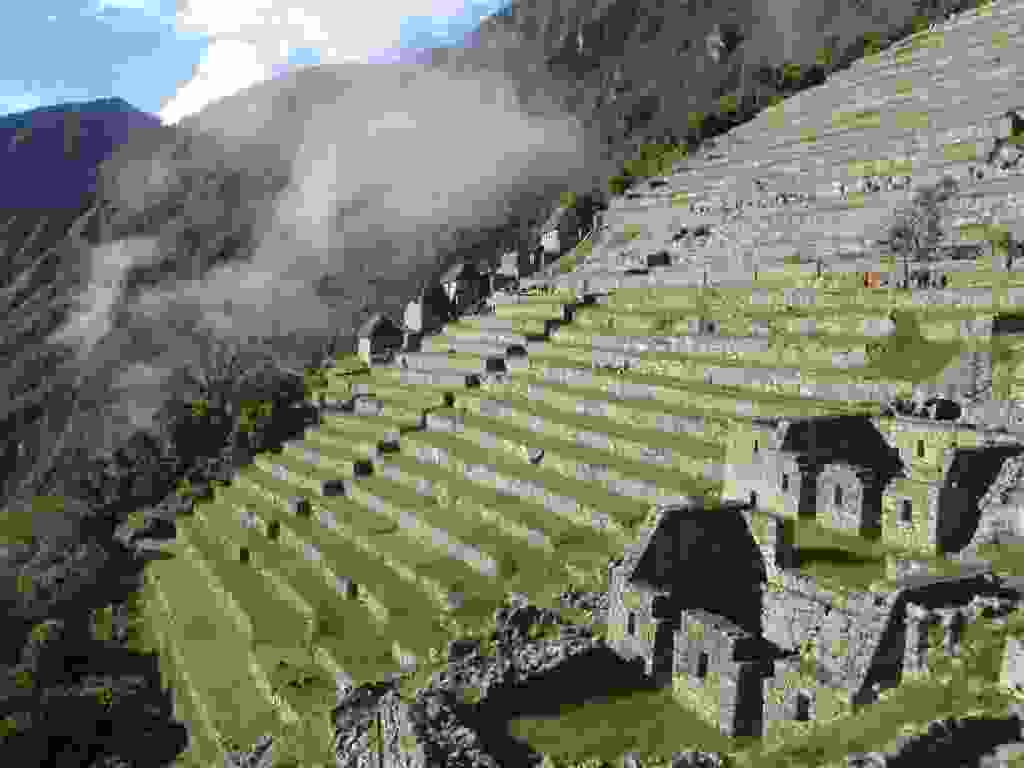
\includegraphics[width=\mywidth]{../wp-content/uploads/2015/06/P5274490-1024x768.jpg} \end{center}
\begin{center} 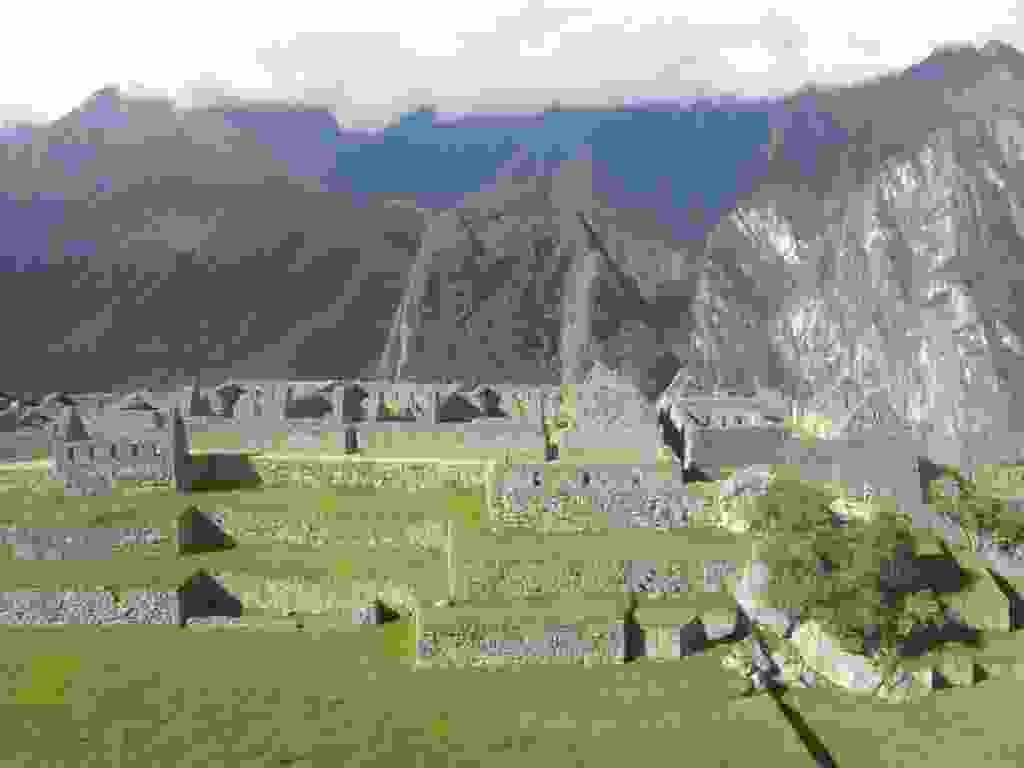
\includegraphics[width=\mywidth]{../wp-content/uploads/2015/06/P5274548-1024x768.jpg} \end{center}
\vspace{-\topsep}
\vspace{-3.25mm}
\pagebreak
~\\
\begin{center} 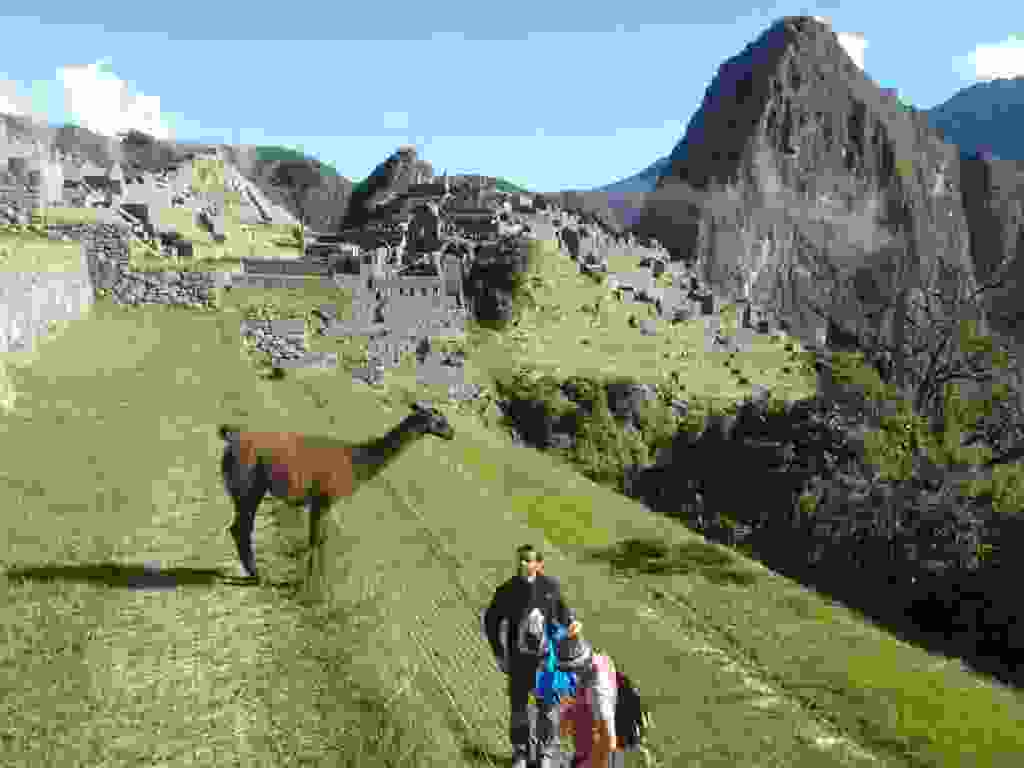
\includegraphics[width=\mywidth]{../wp-content/uploads/2015/06/P5274496-1024x768.jpg} \end{center}

La photo avant de dire au revoir à notre guide. 
\begin{center} 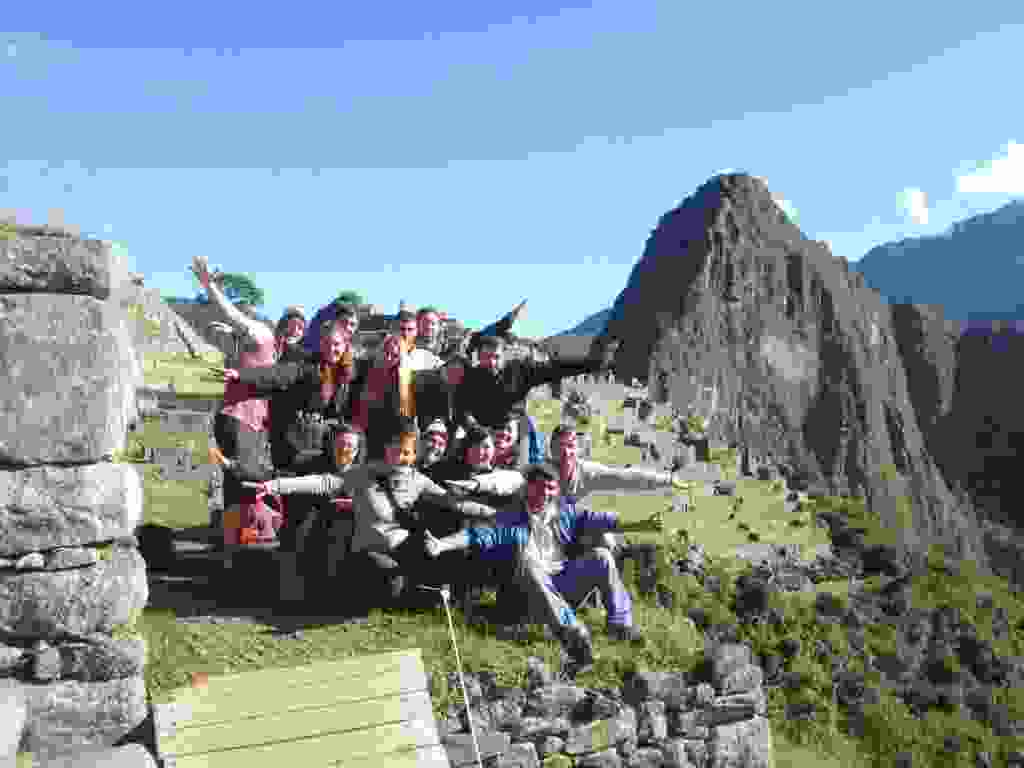
\includegraphics[width=\mywidth]{../wp-content/uploads/2015/06/P5274493-1024x768.jpg} \end{center}
\vspace{-\topsep}
\pagebreak

On monte ensuite en haut de la montagne du Machu Picchu : 1h30 de marches en pierre. 
\begin{center} 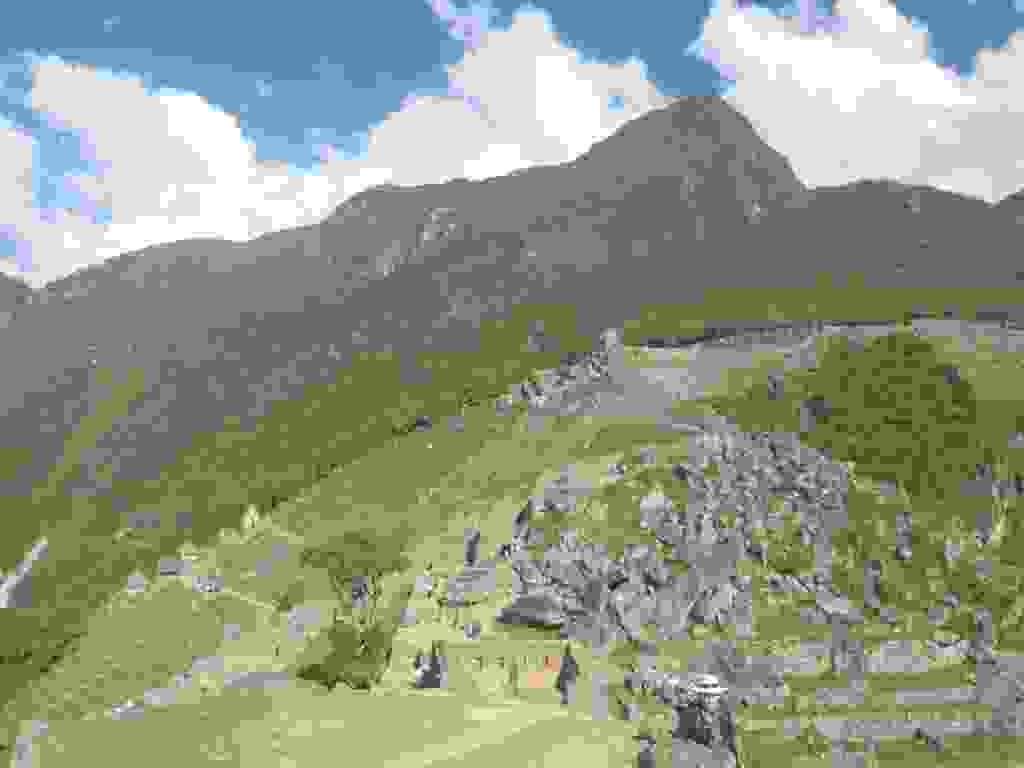
\includegraphics[width=\mywidth]{../wp-content/uploads/2015/06/P5274549-1024x768.jpg} \end{center}
~
\begin{center} 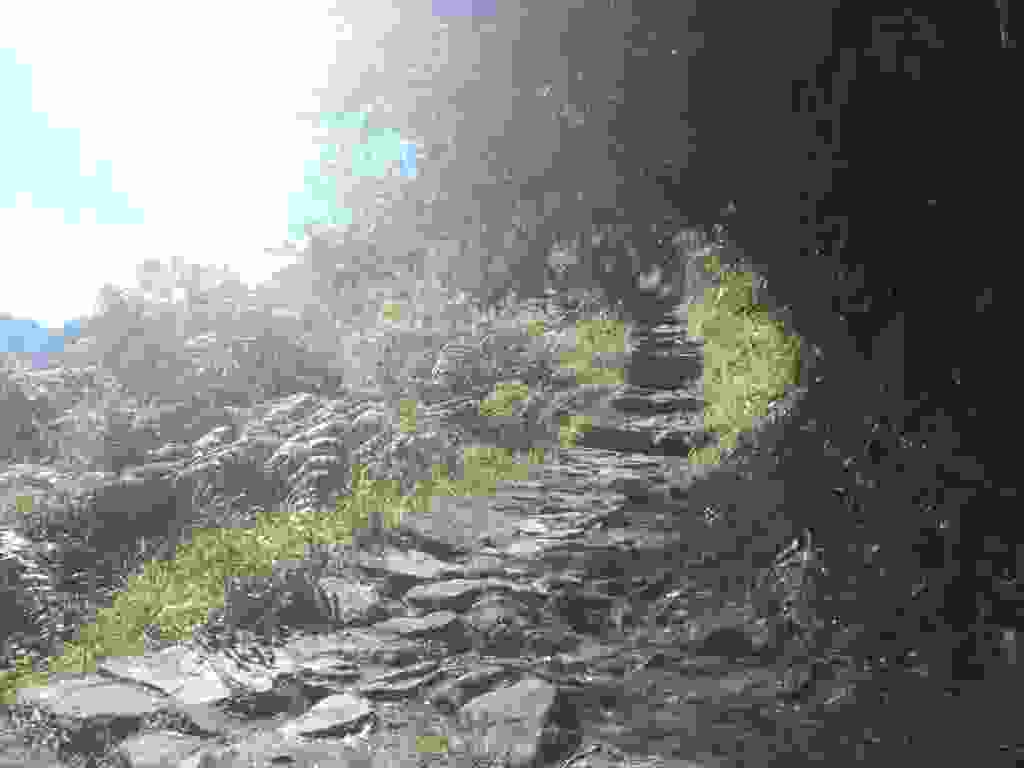
\includegraphics[width=\mywidth]{../wp-content/uploads/2015/06/P5274507-1024x768.jpg} \end{center}
\vspace{-\topsep}
\pagebreak

D'en haut, la vue est grandiose.
\begin{center} 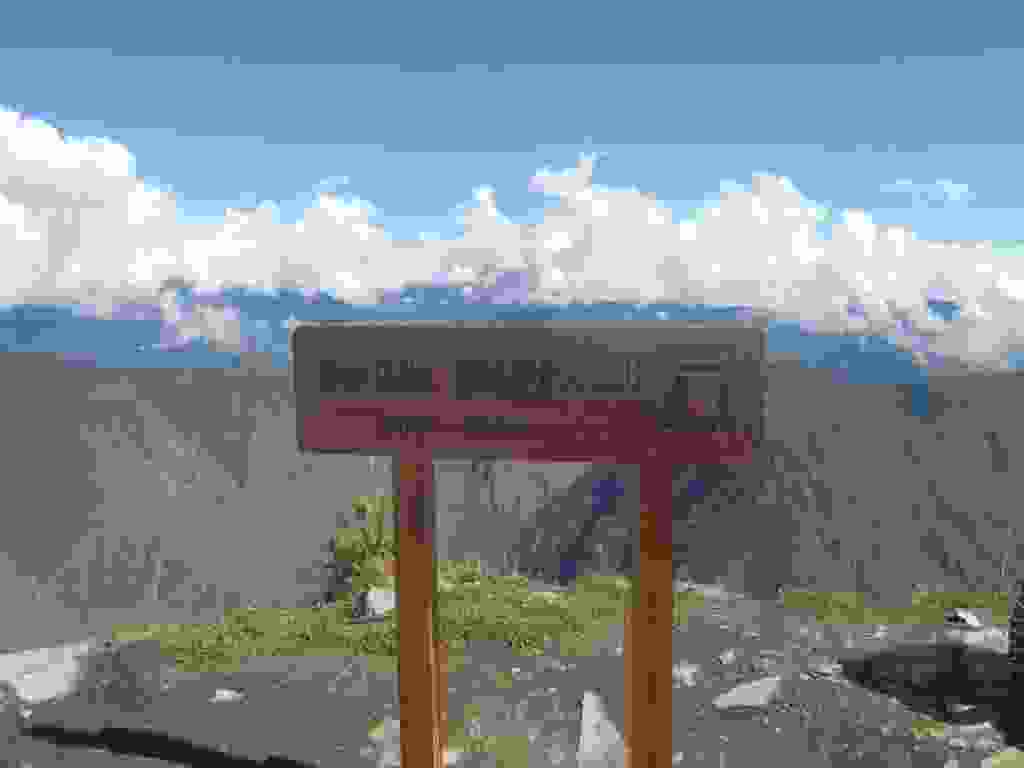
\includegraphics[width=\mywidth]{../wp-content/uploads/2015/06/P5274513-1024x768.jpg} \end{center}
\begin{center} \includegraphics[width=\mywidth]{../wp-content/uploads/2015/06/P5274511-1024x768.jpg} \end{center}
\vspace{-\topsep}
\vspace{-3.25mm}
\pagebreak
~
\begin{center} \includegraphics[width=\mywidth]{../wp-content/uploads/2015/06/P5274508-1024x768.jpg} \end{center}
\begin{center} \includegraphics[width=\mywidth]{../wp-content/uploads/2015/06/P5274509-1024x768.jpg} \end{center}

\begin{center} \includegraphics[height=\mywidth]{../wp-content/uploads/2015/06/P5274521-768x1024.jpg} \end{center}
\vfill
\begin{center} \includegraphics[width=\mywidth]{../wp-content/uploads/2015/06/P5274515-1024x768.jpg} \end{center}
\vspace{-\topsep}
\vspace{-0.75mm}
\pagebreak

Le pont inca à 20 min de marche. 
\begin{center} \includegraphics[width=\mywidth]{../wp-content/uploads/2015/06/P5274537-1024x768.jpg} \end{center}

\subsection*{Jour 6}
Retour à Hidroelectrica par la voie ferrée puis 7h de bus pour rentrer à Cusco.
